\title{CS313 : DataBases and Information Systems Lab\\
    \vspace{0.6cm}
    Project 2
} % You may change the title if you want.
% \subtitle{Hello}
\author{Sourabh Bhosale (200010004) \\ \vspace{7mm}
        Dibyashu Kashyap (200010013)}

\date{\today}

\documentclass[12pt]{article}
\usepackage{fullpage}
\usepackage{enumitem}
\usepackage{amsmath,mathtools}
\usepackage{amssymb}
\usepackage[super]{nth}
\usepackage{textcomp}
\usepackage{hyperref}
\usepackage{multicol}
\usepackage{multirow}
\usepackage{minted}
\usepackage{xcolor}
\usepackage{setspace}
% \usepackage{fontspec}
% \usepackage[showframe]{geometry}

% \usepackage[default,oldstyle,scale=0.95]{helvet}
% \usepackage[T1]{fontenc}

% \usepackage{merriweather}
% \usepackage[T1]{fontenc}

% \usepackage[sfdefault]{noto}
% \usepackage[T1]{fontenc}
\definecolor{bgcolor}{HTML}{E0E0E0}
\let\oldtexttt\texttt
\renewcommand{\texttt}[1]{
  \colorbox{bgcolor}{\oldtexttt{#1}}
  }

\usepackage[default,oldstyle,scale=0.95]{opensans}
%% Alternatively use the option 'defaultsans' instead of 'default' to 
%% replace the sans serif font only.
\usepackage[T1]{fontenc}

% \usepackage[scaled]{helvet} 
% \setmainfont{Roboto}
\usepackage{titling}
\hypersetup{
    colorlinks=true,
    linkcolor=blue,
    filecolor=magenta,      
    urlcolor=cyan,
}

\renewcommand\maketitlehooka{\null\mbox{}\vfill}
\renewcommand\maketitlehookd{\vfill\null}

\begin{document}

\begin{titlingpage}
\maketitle
\end{titlingpage}

\newpage
%---------------------------------------------------------------------
\section{Overview of the project}

\textbf{Hospital Management System:}
\vspace{5mm} \\

This is a system that has the following functionalities:

\begin{itemize}
    \item Add new doctor
    \item Add new patient
    \item Add new staff
    \item Book an appointment option for admin
    \item Book an appointment option for patient
    \item Updating details option for doctor
    \item View personal details option for doctor
    \item View personal details option for patient
\end{itemize}

This hospital management system can be used by people who needs treatment according to the allergies or disease they have. First they will have to register themselves as a patient through admin, where they have to give all the information about themselves like name, address, allergies, height, weight etc. Then appointment can be booked by admin or patient can do it by himself after logging in.
We also have an option to add a doctor or hospital staff by taking respective information like name, department names they want to work in, speciality for doctor. Doctor can update his details later on if required. And doctor and patient can view the details of themselves after logging in.

\newpage

%---------------------------------------------------------------------
\section{Database schema, ER Model, Integrity Constraints and views,
Users}

\subsection{Database schema and Integrity Constraints}

\begin{table}[!hbt]
    \centering
    \begin{tabular}{|c|c|c|c|c|} 
        \hline
        \textbf{Table} & \textbf{Primary Key} & \textbf{Domain of P.K.} & 
        \textbf{
        \begin{tabular}[c]{@{}c@{}}Foreign keys\\(Referencing table) \end{tabular}} & \textbf{Not Null} \\ 
        \hline\hline
        patient & patient\_id & VARCHAR & - & - \\ 
        \hline
        address &  patient\_id  & VARCHAR & patient\_id references patient  & - \\
        \hline
        allergies &  patient\_id  & VARCHAR & patient\_id references patient  & - \\
        \hline
        dept & dept\_name & VARCHAR & - & - \\
        \hline
        doctor & doctor\_id & VARCHAR & dept\_name references dept  & - \\
        \hline
        staff & staff\_id & VARCHAR & dept\_name references dept  & - \\
        \hline
        appointment & 
        appointment\_id & 
        VARCHAR & 
        \begin{tabular}[c]{@{}c@{}}patient\_id references patient\\doctor\_id references doctor \end{tabular} 
        & - \\
        \hline
        adminpass & 
        \begin{tabular}[c]{@{}c@{}}admin\_id \\  \end{tabular} & 
        VARCHAR & 
        -
        & - \\
        \hline
        docpass & 
        \begin{tabular}[c]{@{}c@{}}doc\_id \\ pass \end{tabular} & 
        VARCHAR& 
        \begin{tabular}[c]{@{}c@{}}doctor\_id references doctor\\doctor\_id references doctor \end{tabular} 
        & - \\
        \hline
        patpass & 
        \begin{tabular}[c]{@{}c@{}}\\ patient\_id \\ pass \end{tabular} & 
        VARCHAR & 
        \begin{tabular}[c]{@{}c@{}}patient\_id references patient \\ patient\_id references patient \end{tabular}
        & - \\
        \hline  
    \end{tabular}
    \caption{Table of constraints}
    \label{tab:my_label}
\end{table}

\subsection{Users}

There are 3 types of users in our hospital management system:

\begin{itemize}
    \item Admin :
    An admin after loging-in  with the correct credentials can add a new doctor, new patient, new staff and an appointment for a patient.  
    \item Doctor :
     A doctor after loging-in  with the correct credentials can update his/her details and also view his/her details.
    \item Patient :
     A patient after loging-in  with the correct credentials can add an appointment and also view the details.
\end{itemize}

\newpage
\subsection{ER Model}

\begin{figure}[!hbt]
    \centering
    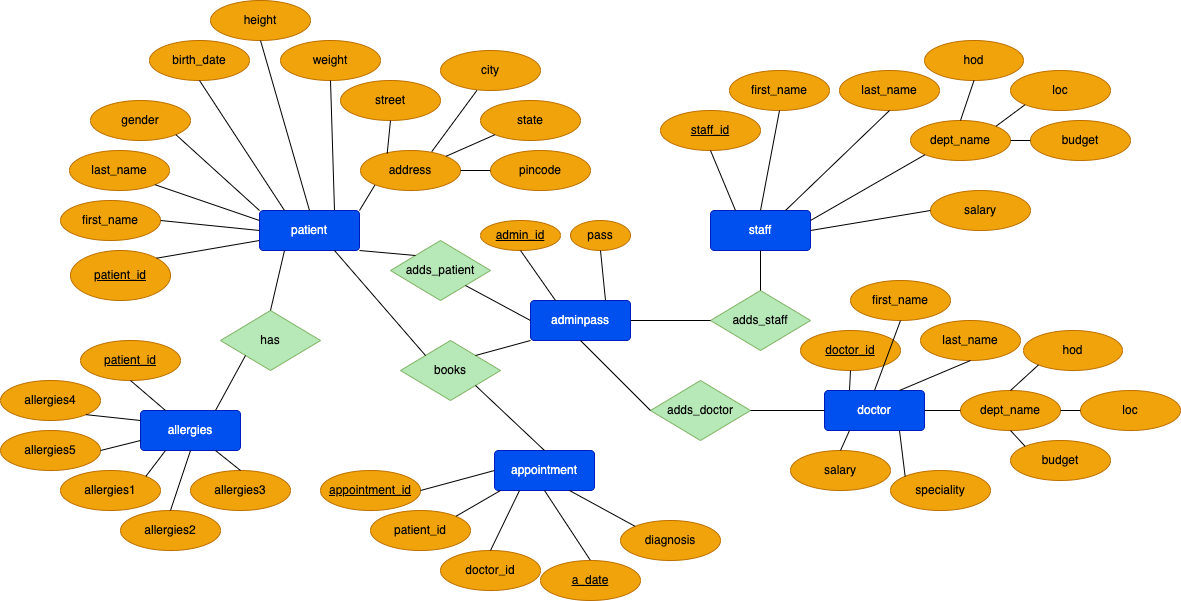
\includegraphics[scale=0.43]{er.png}
    \label{fig:data}
    \caption{ER Diagram}
\end{figure}

\newpage
%---------------------------------------------------------------------
\section{Relational Database design(Tables creation)}

\begin{figure}[!hbt]
    \centering
    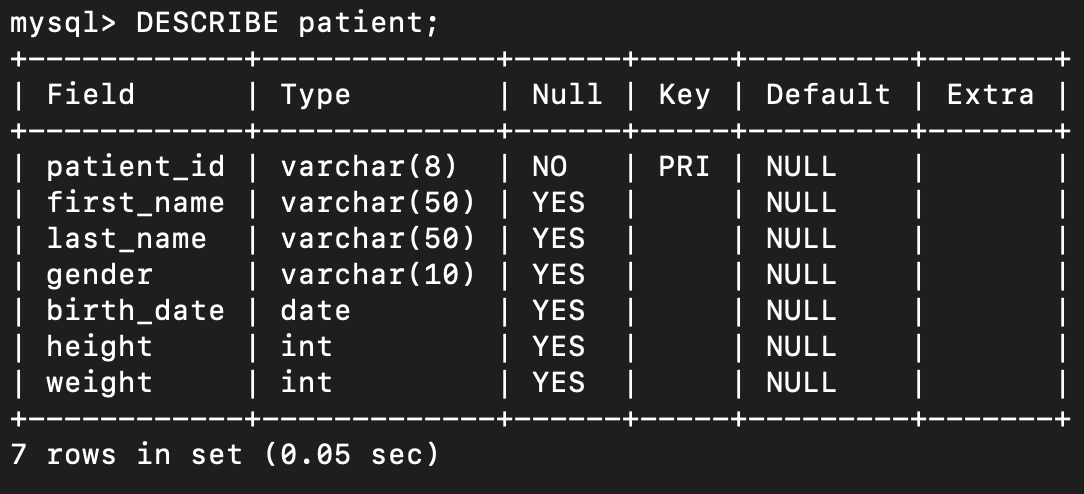
\includegraphics[scale=0.85]{tables/1.png}
    \label{fig:data}
    \caption{\texttt{patient} table}
\end{figure}

\vspace{5mm}

\begin{figure}[!hbt]
    \centering
    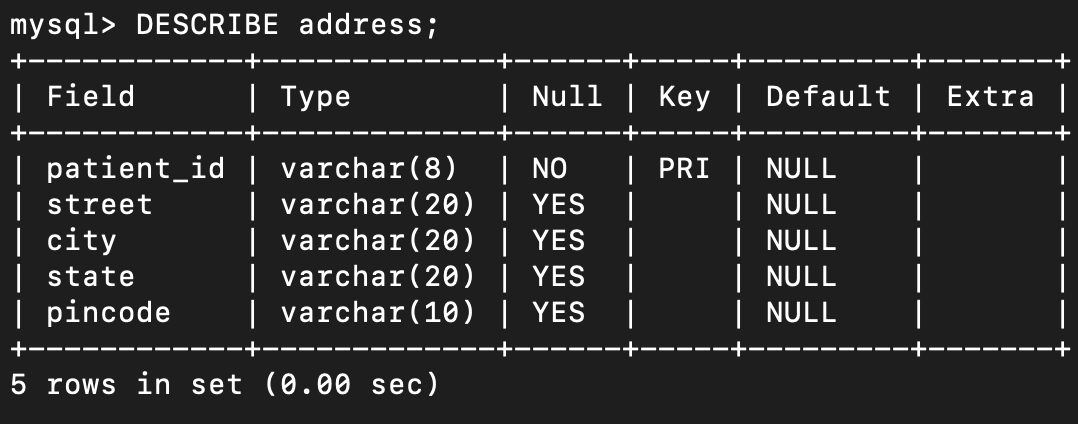
\includegraphics[scale=0.85]{tables/2.png}
    \label{fig:my_label1}
    \caption{\texttt{address} table}
\end{figure}

\newpage

\begin{figure}[!hbt]
    \centering
    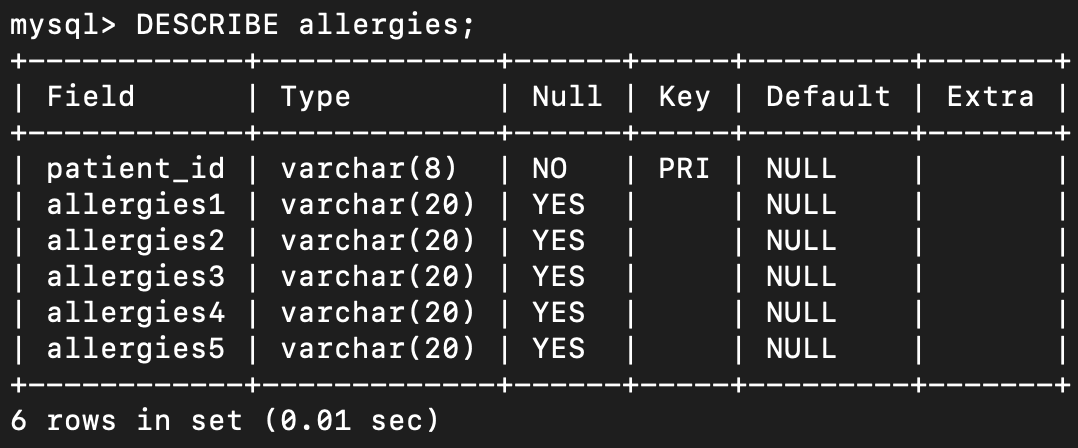
\includegraphics[scale=0.85]{tables/3.png}
    \label{fig:data}
    \caption{\texttt{allergies} table}
\end{figure}

\vspace{5mm}

\begin{figure}[!hbt]
    \centering
    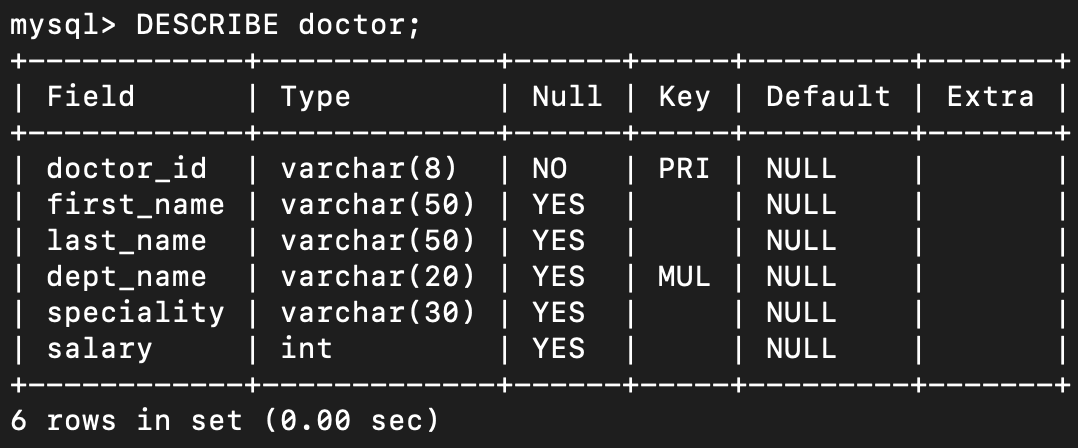
\includegraphics[scale=0.85]{tables/4.png}
    \label{fig:my_label1}
    \caption{\texttt{doctor} table}
\end{figure}

\newpage

\begin{figure}[!hbt]
    \centering
    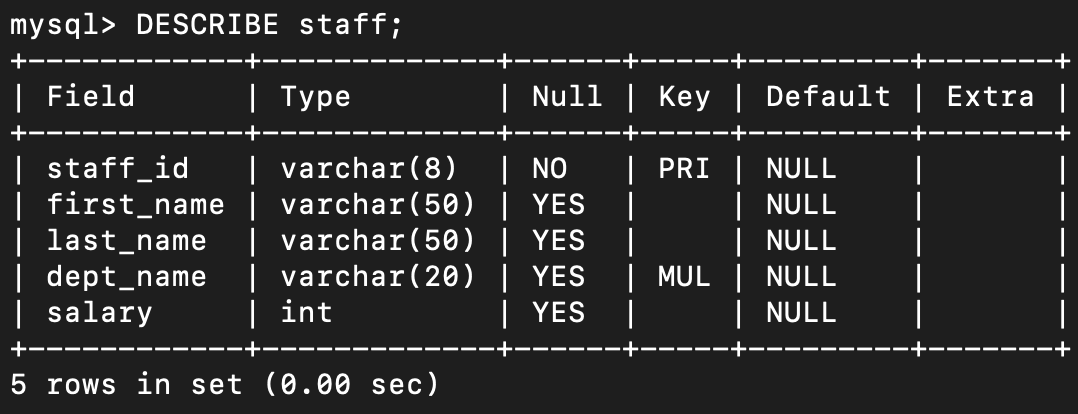
\includegraphics[scale=0.85]{tables/5.png}
    \label{fig:data}
    \caption{\texttt{staff} table}
\end{figure}

\vspace{5mm}

\begin{figure}[!hbt]
    \centering
    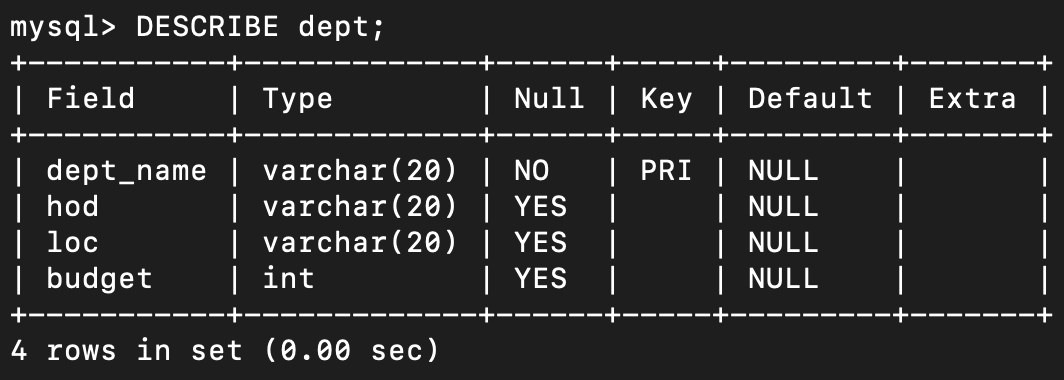
\includegraphics[scale=0.85]{tables/6.png}
    \label{fig:my_label1}
    \caption{\texttt{dept} table}
\end{figure}

\newpage

\begin{figure}[!hbt]
    \centering
    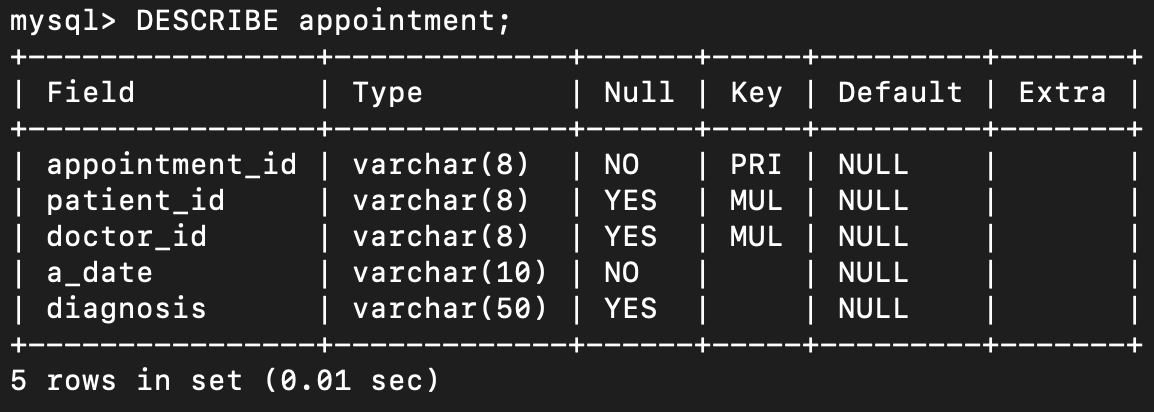
\includegraphics[scale=0.85]{tables/7.png}
    \label{fig:data}
    \caption{\texttt{appointment} table}
\end{figure}

\vspace{5mm}

\begin{figure}[!hbt]
    \centering
    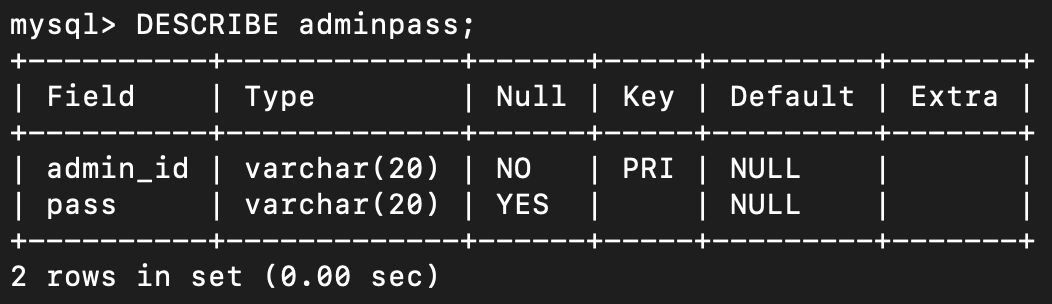
\includegraphics[scale=0.85]{tables/8.png}
    \label{fig:my_label1}
    \caption{\texttt{adminpass} table}
\end{figure}

\newpage

\begin{figure}[!hbt]
    \centering
    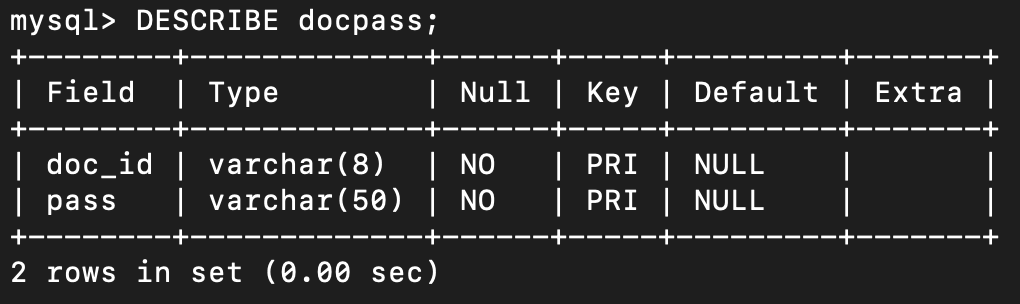
\includegraphics[scale=0.85]{tables/9.png}
    \label{fig:data}
    \caption{\texttt{docpass} table}
\end{figure}

\begin{figure}[!hbt]
    \centering
    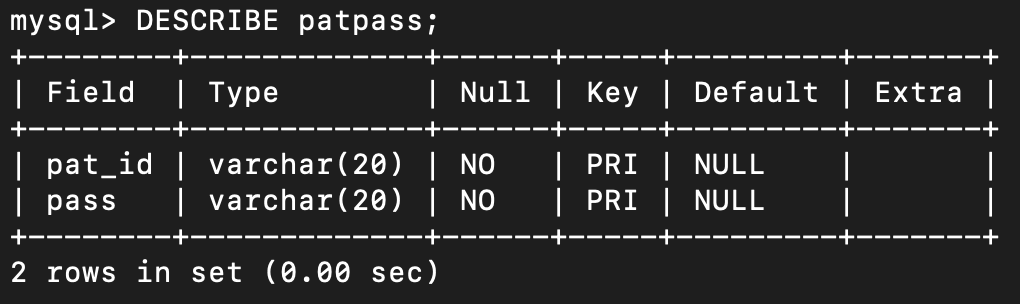
\includegraphics[scale=0.85]{tables/10.png}
    \label{fig:my_label1}
    \caption{\texttt{patpass} table}
\end{figure}

\newpage
%---------------------------------------------------------------------
\section{Languages and Technologies used}

\subsection{Technologies used}
\begin{itemize}
    \item Eclipse IDE
    \item Visual Studio Code
    \item Java JDBC
    \item J2EEE
    \item MySQL Database 
    \item Servlets and JSP files. 
    \item Apache Tomcat 8.5 Server
\end{itemize}

\subsection{Languages used}
\begin{itemize}
    \item Java (for Servlets)
    \item HTML in JSP files
    \item CSS
    \item MySQL
    \item XML
\end{itemize}

\subsection{Libraries used}
\begin{itemize}
    \item Bootstrap CSS Library
    \item MySQL Library (.jar)
\end{itemize}

% \newpage
%---------------------------------------------------------------------
\section{Interface Designs}

In this hospital management system, we have used vanilla css along with the bootstrap library, HTML fields and buttons for text fields and referencing different pages.

\newpage
%---------------------------------------------------------------------
\section{Workflow and Pages}

\begin{itemize}
    \item At start, we will be at Home page (\texttt{Home.jsp}) where different options like Admin login, Doctor Login, Patient Login will be there.
    \item First let's look into Admin login (\texttt{adminlog.jsp}), if we enter correct login credentials, then it will proceed further and give options like Add a doctor, Add a patient, Add a staff and Book an appointmnt using \texttt{AdminlogServlet}.
    \item But if the login credentials are incorrect, then it will show error message to enter the correct ones.
    \item Admin can add a doctor (\texttt{adddoc.jsp}), add a patient (\texttt{addpat.jsp}), add a staff (\texttt{addstaff.jsp}) and book an appointment (\texttt{addapp.jsp}). Each of the things will be controlled by servlet files like (\texttt{AdddocServlet.java}), (\texttt{AddpatServlet.java}), (\texttt{AddstaffServlet.java}) and (\texttt{AddappServlet.java})
    \item For each of the things, primary key constraints should be followed and if not it will show error message.
    \item Now, let's have a look at Doctor login (\texttt{doclog.jsp}), if we enter correct login credentials, then it will proceed further and give options like update the details (\texttt{updatedoc.jsp}) and show the details (\texttt{showdoc.jsp}) using (\texttt{DoctorlogServlet}). For updating details, sure to follow primary key constraints and if not it will show error message.
    \item But if the login credentials are incorrect for doctor, then it will show error message to enter the correct ones.
    \item Now for the Patient login (\texttt{patlog.jsp}), if we enter correct login credentials, then it will proceed further and give options like book an appointment (\texttt{addapp.jsp} and show the details (\texttt{showpat.jsp} using (\texttt{PatientlogServlet.java}). For booking an appointment, make sure to follow primary key constraints and if not it will show error message.
    \item  If the login credentials are incorrect for patient, then it will show error message to enter the correct ones.
\end{itemize}
\newpage
%---------------------------------------------------------------------
\section{Add the relevant Screenshots}

\begin{figure}[!hbt]
    \centering
    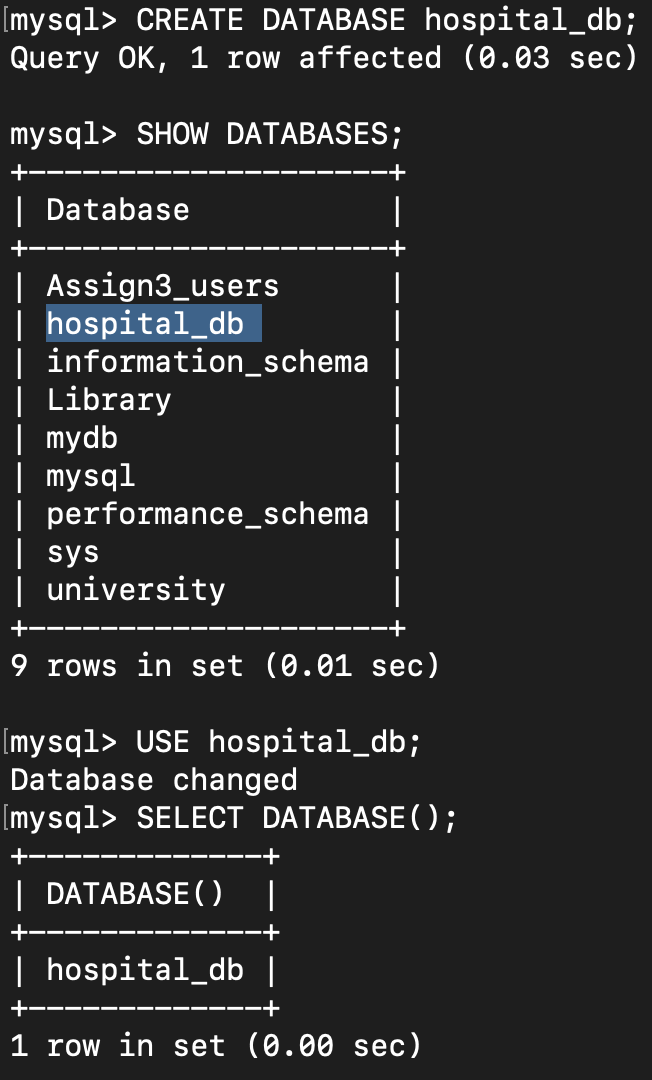
\includegraphics[scale=0.55]{screenshots/1a.png}
    \label{fig:data}
    \caption{Creating new database \texttt{hospital\_db}}
\end{figure}

\begin{figure}[!hbt]
    \centering
    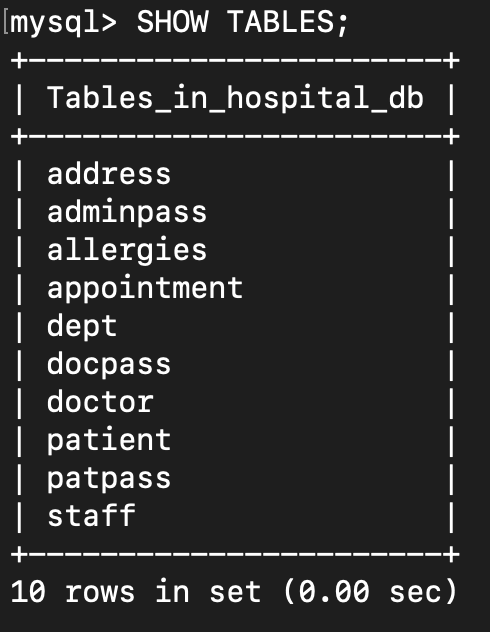
\includegraphics[scale=0.55]{screenshots/1b.png}
    \label{fig:my_label1}
    \caption{Tables inside \texttt{hospital\_db}}
\end{figure}

\newpage

\begin{figure}[!hbt]
    \centering
    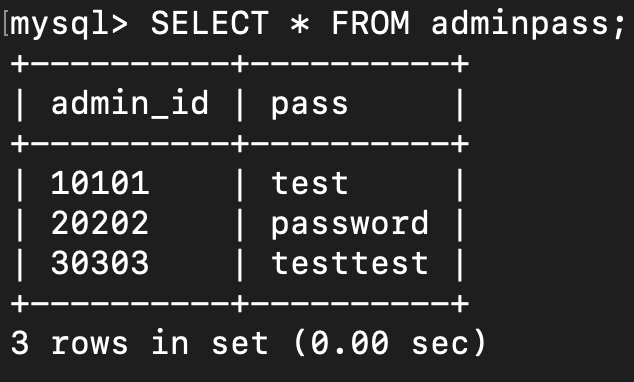
\includegraphics[scale=1.0]{screenshots/1c.png}
    \label{fig:data}
    \caption{Credentials present for Admin login in the database}
\end{figure}

\begin{figure}[!hbt]
    \centering
    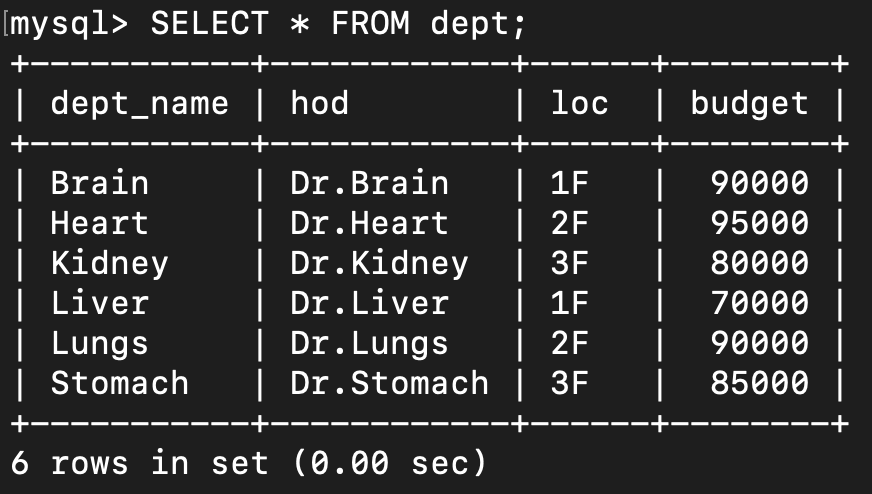
\includegraphics[scale=1.0]{screenshots/1d.png}
    \label{fig:my_label1}
    \caption{Initially inserted department table values}
\end{figure}

\newpage

\begin{figure}[!hbt]
    \centering
    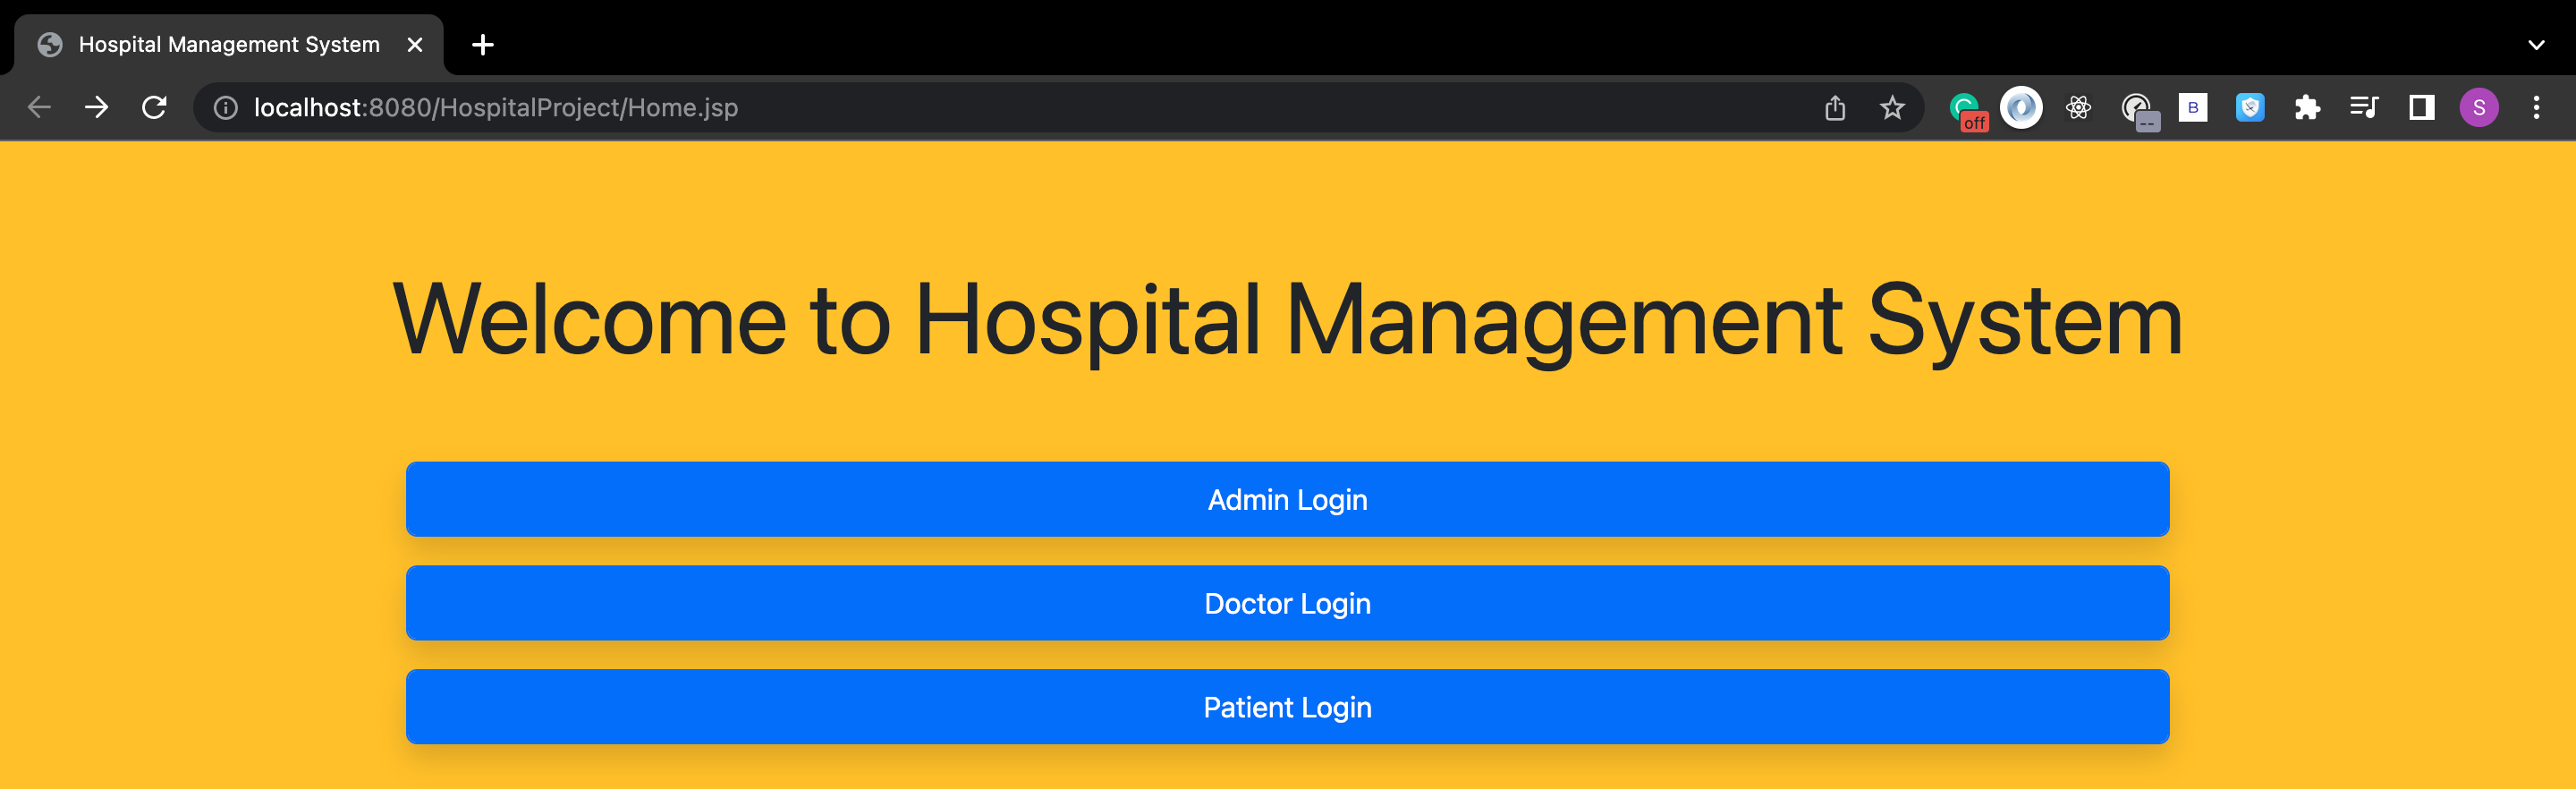
\includegraphics[scale=0.35]{screenshots/2a.png}
    \label{fig:data}
    \caption{Home page}
\end{figure}

\vspace{15mm}

\begin{figure}[!hbt]
    \centering
    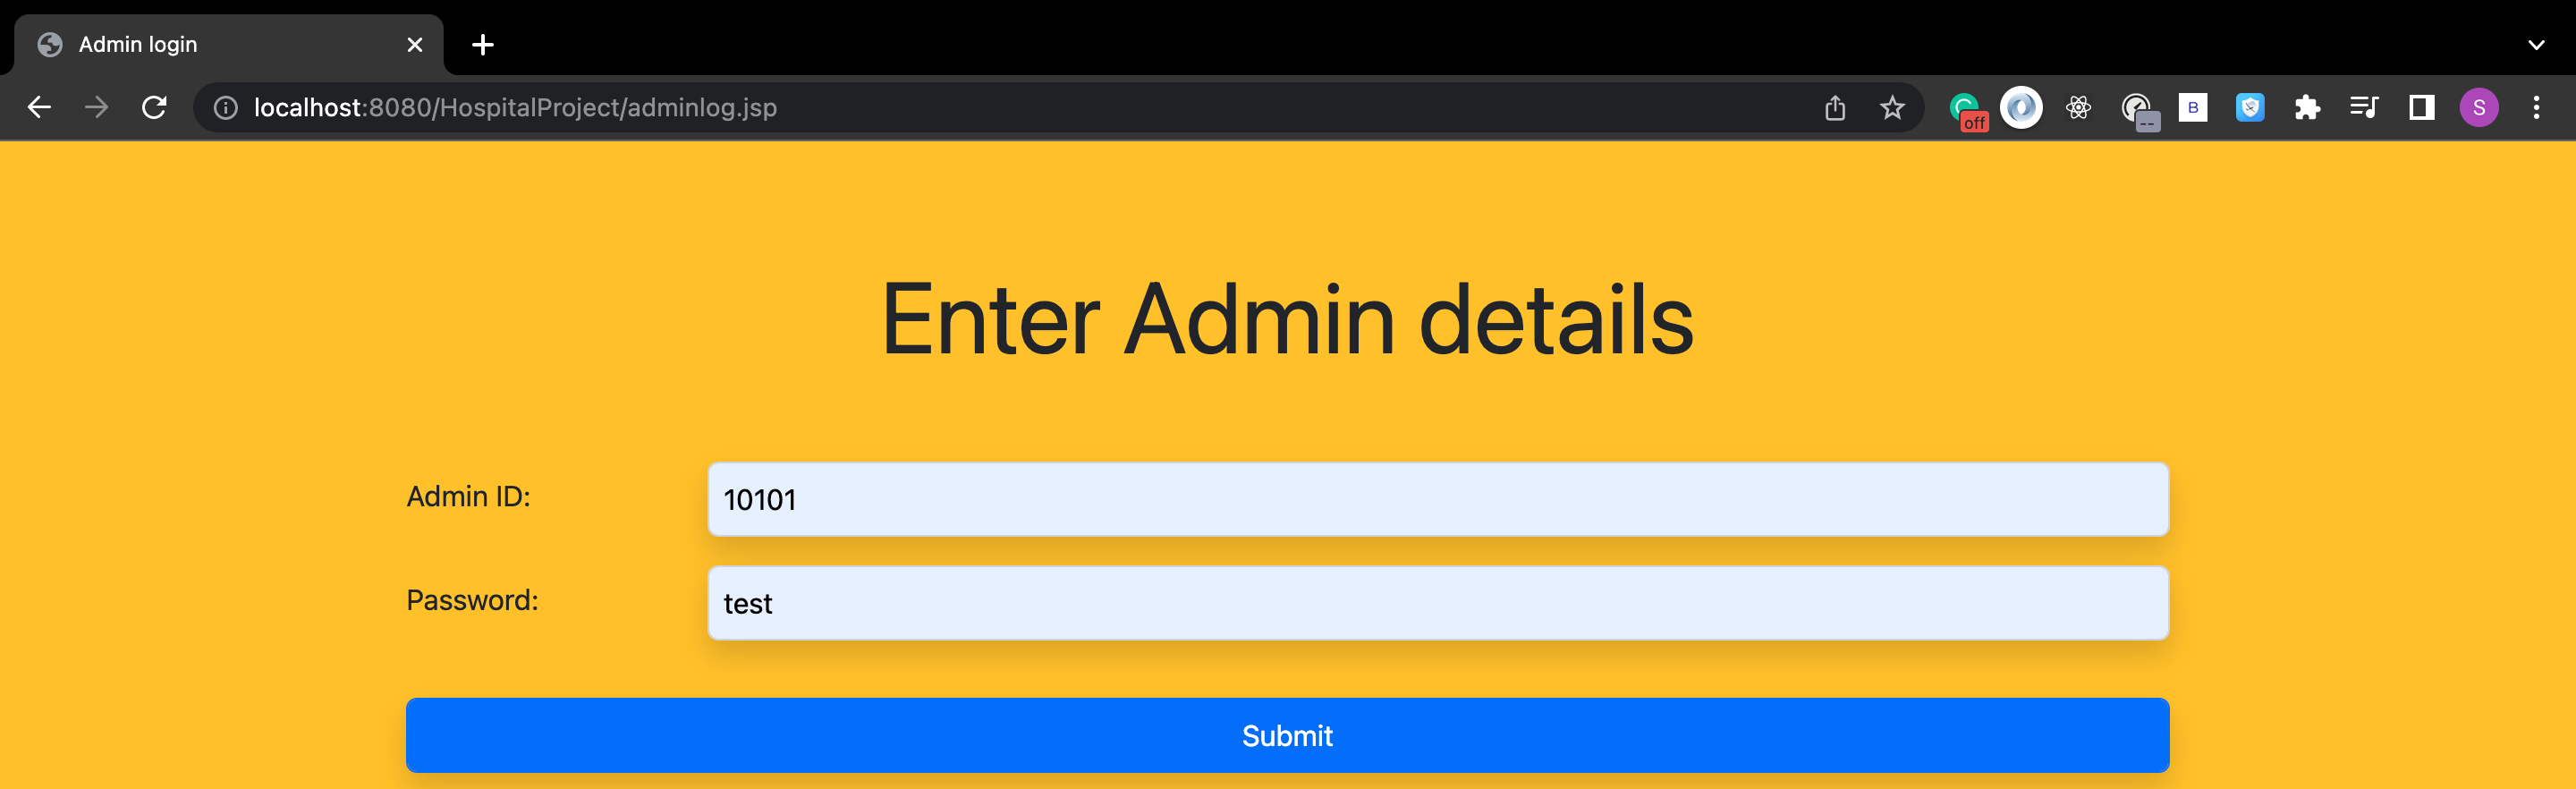
\includegraphics[scale=0.35]{screenshots/2b.png}
    \label{fig:my_label1}
    \caption{Admin login page(using correct credentials)}
\end{figure}

\newpage

\begin{figure}[!hbt]
    \centering
    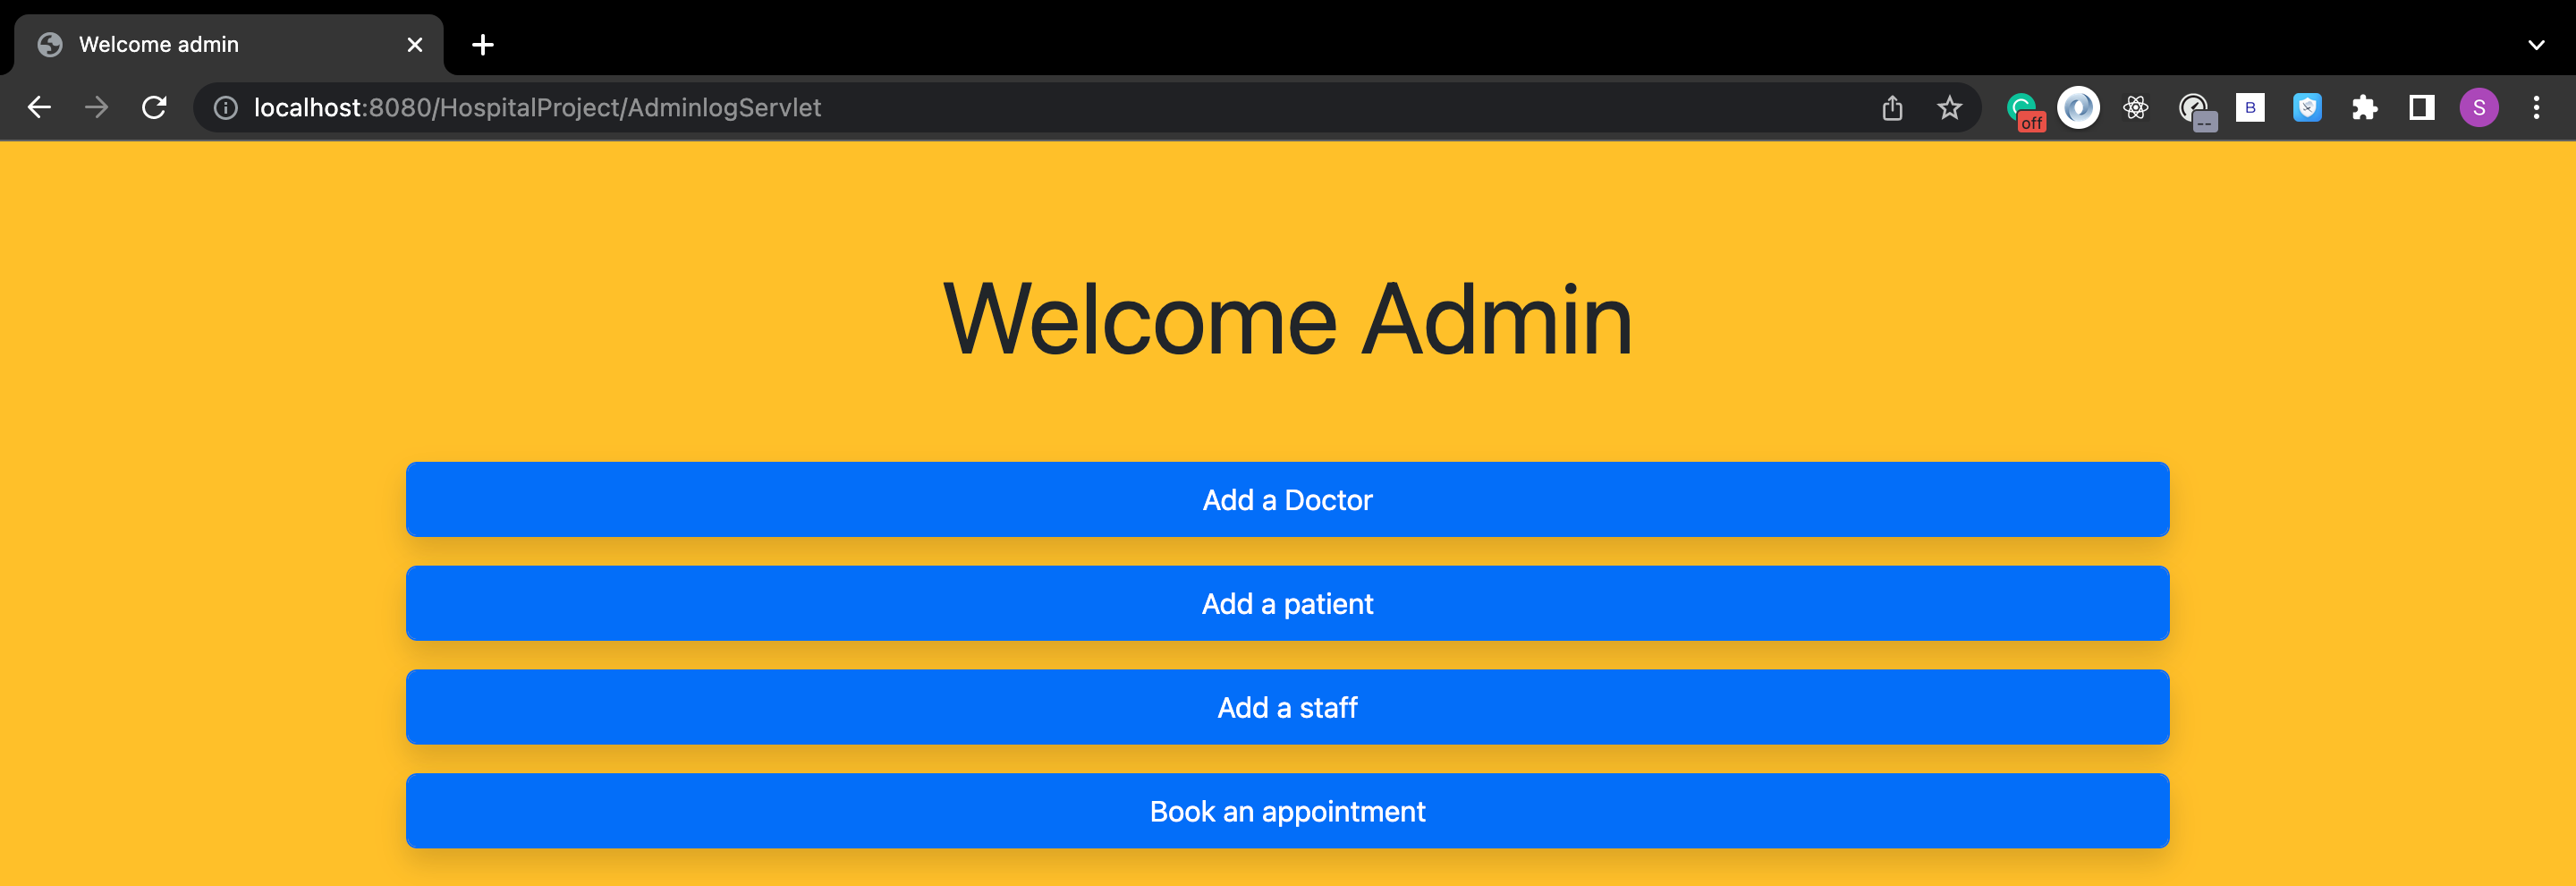
\includegraphics[scale=0.35]{screenshots/2c.png}
    \label{fig:data}
    \caption{Page after successful admin login}
\end{figure}

\begin{figure}[!hbt]
    \centering
    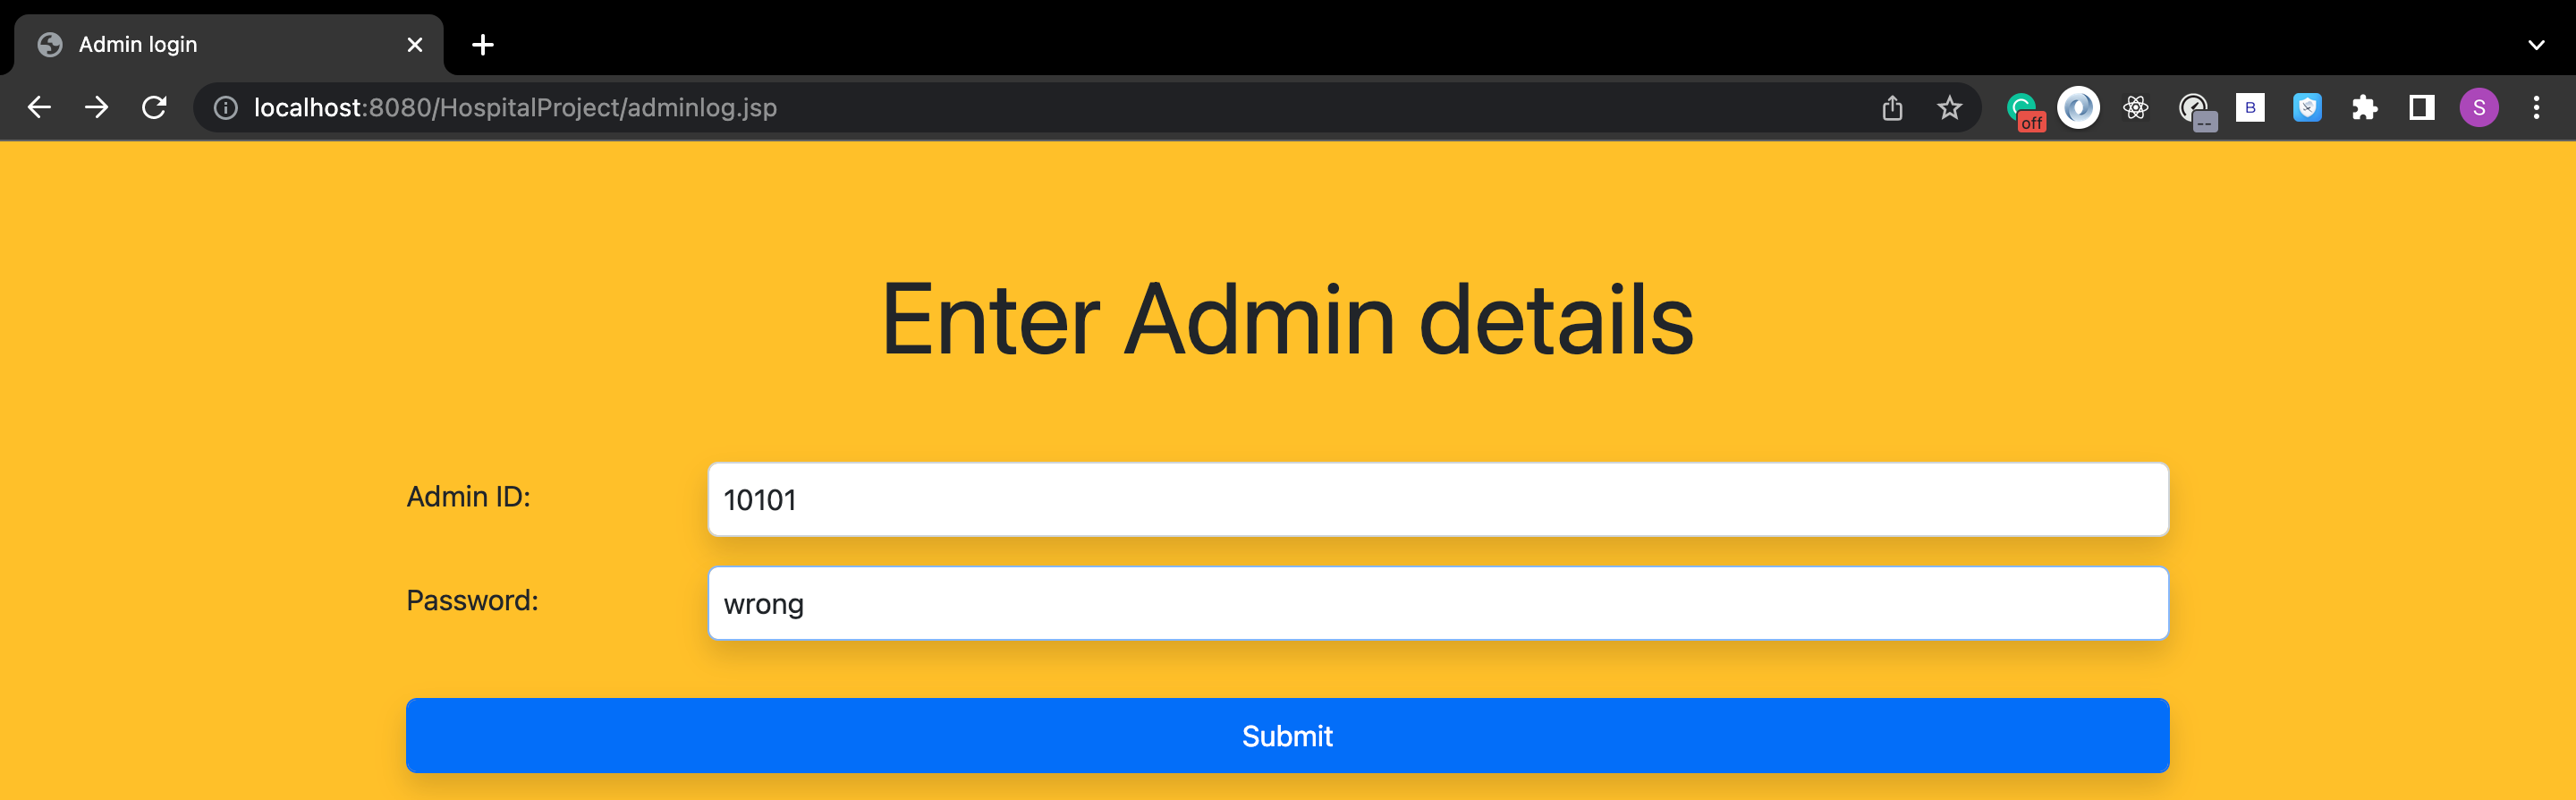
\includegraphics[scale=0.35]{screenshots/2d.png}
    \label{fig:my_label1}
    \caption{Admin login page(using incorrect credentials)}
\end{figure}

\begin{figure}[!hbt]
    \centering
    
\includegraphics[scale=0.8]{screenshots/2e.png}
    \label{fig:data}
    \caption{Result of incorrect login credentials}
\end{figure}

\newpage

\begin{figure}[!hbt]
    \centering
    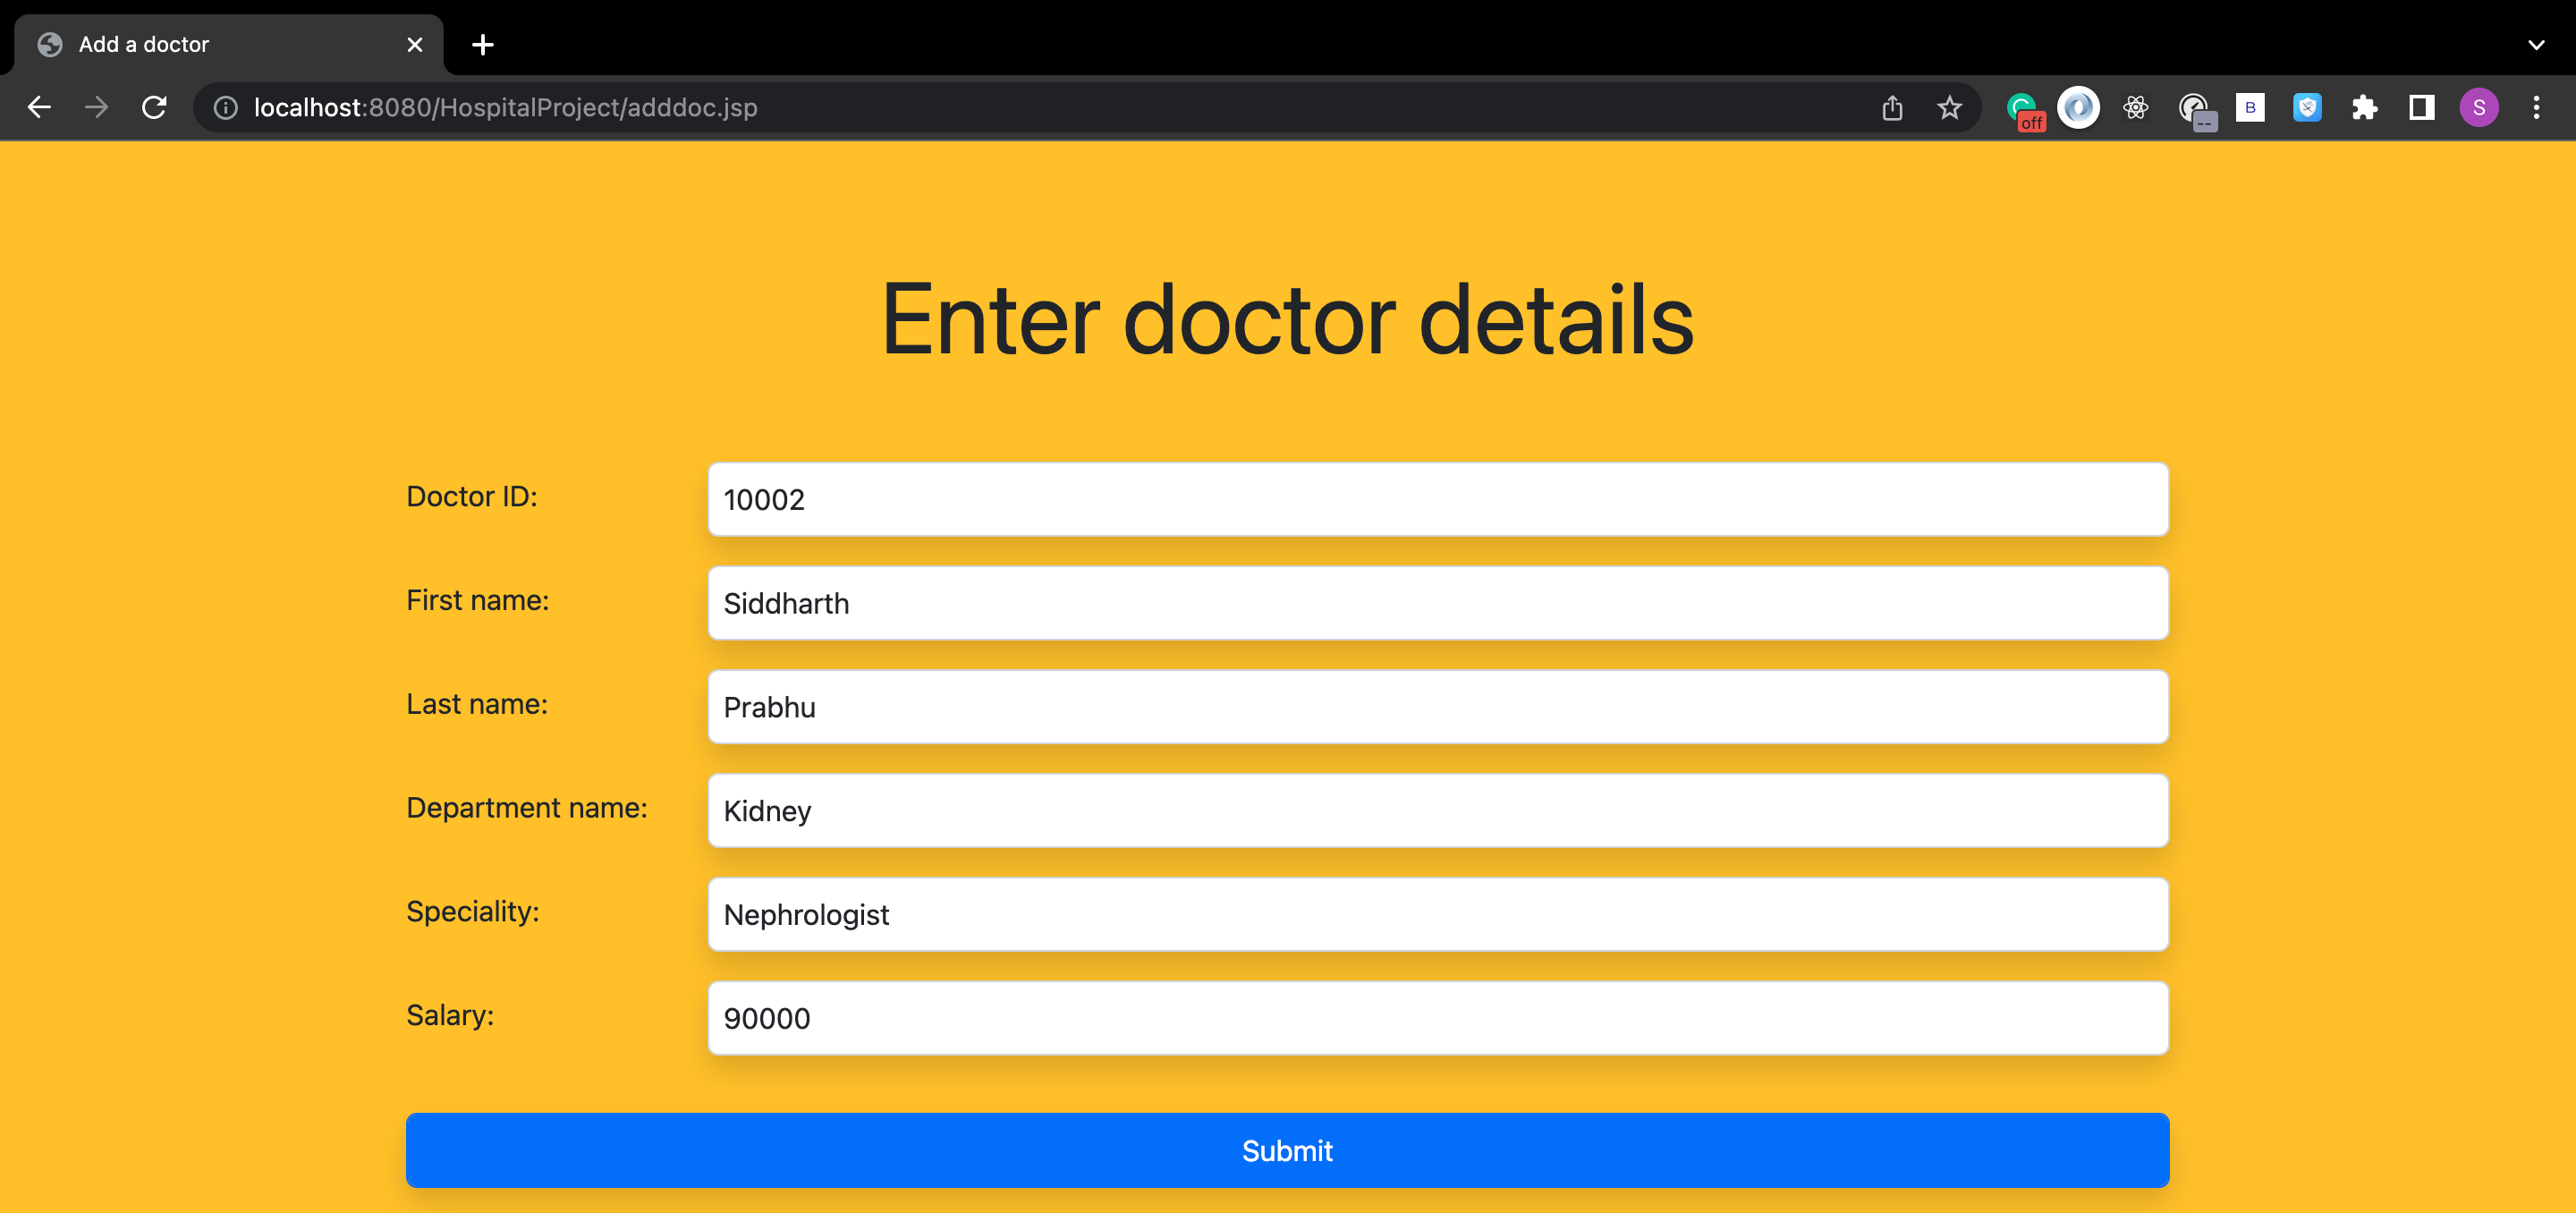
\includegraphics[scale=0.35]{screenshots/2f.png}
    \label{fig:my_label1}
    \caption{Adding a doctor}
\end{figure}

\begin{figure}[!hbt]
    \centering
    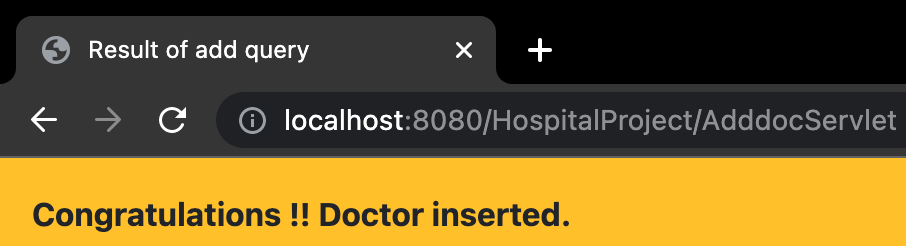
\includegraphics[scale=0.85]{screenshots/2g.png}
    \label{fig:data}
    \caption{Successful insertion of doctor}
\end{figure}

\begin{figure}[!hbt]
    \centering
    
\includegraphics[scale=0.85]{screenshots/2h.png}
    \label{fig:my_label1}
    \caption{Error message if we try to violate the PK constraint}
\end{figure}

\newpage

\begin{figure}[!hbt]
    \centering
    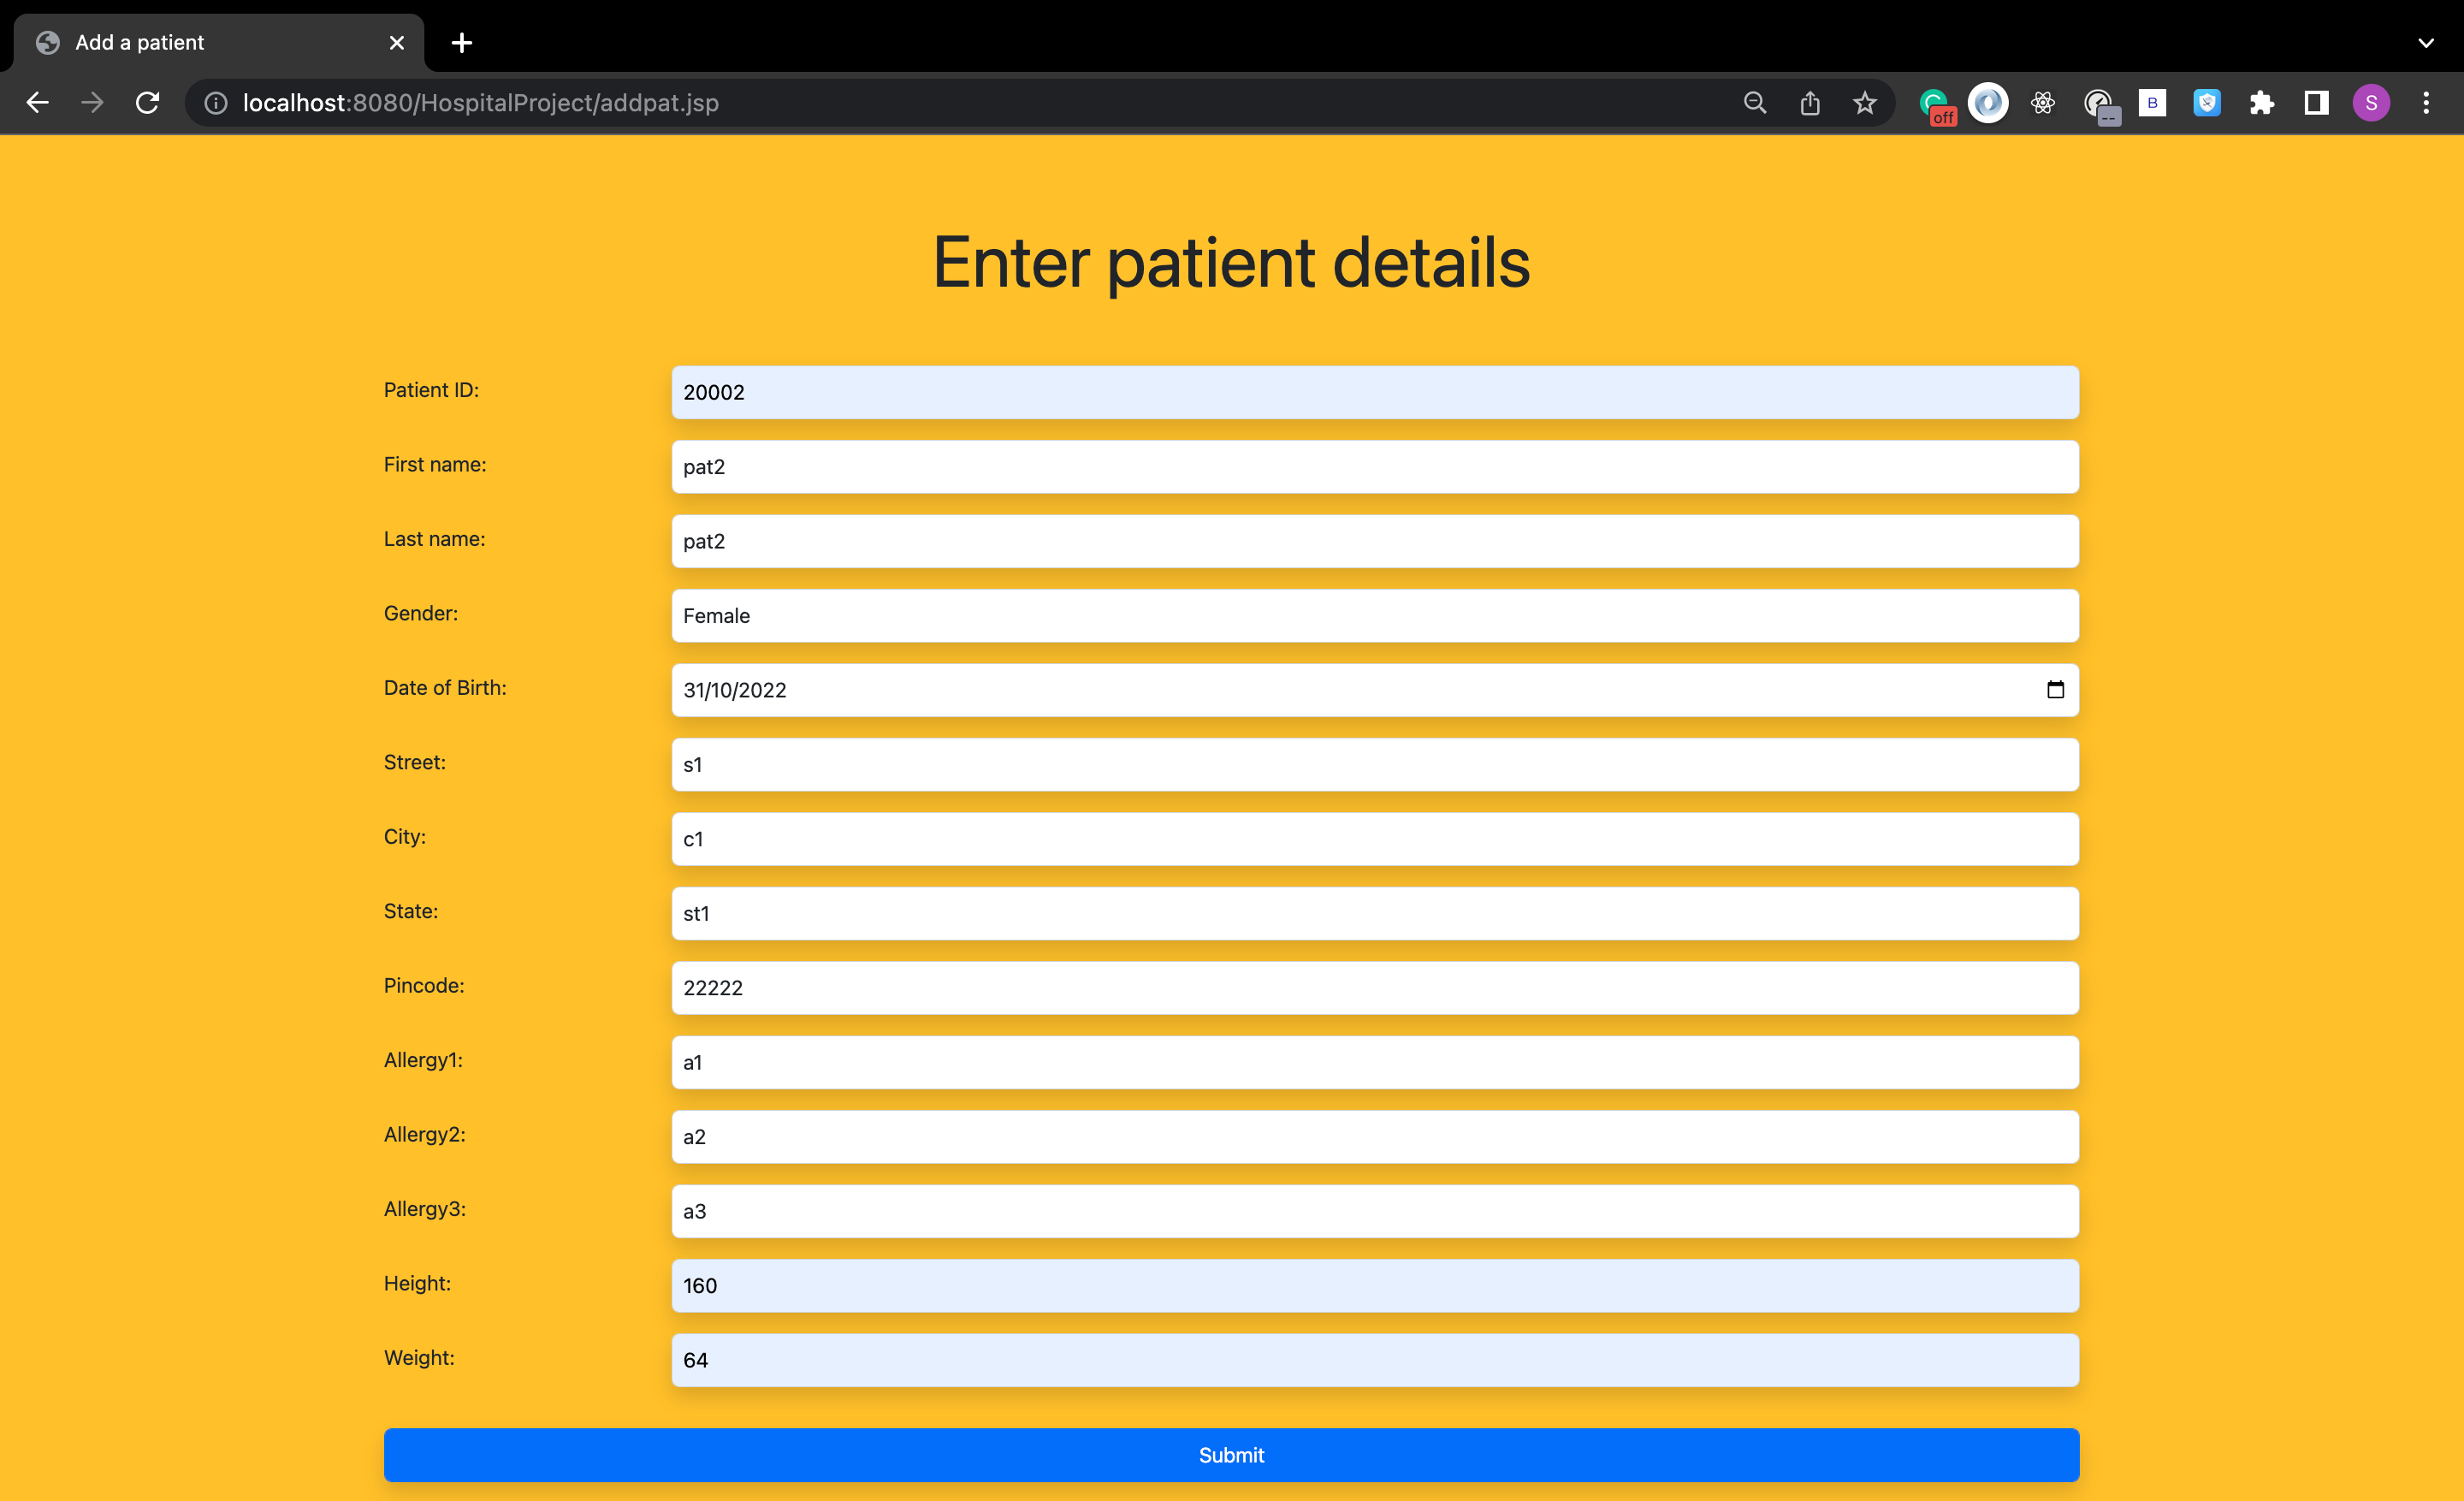
\includegraphics[scale=0.33]{screenshots/2i.png}
    \label{fig:data}
    \caption{Adding a patient}
\end{figure}

\begin{figure}[!hbt]
    \centering
    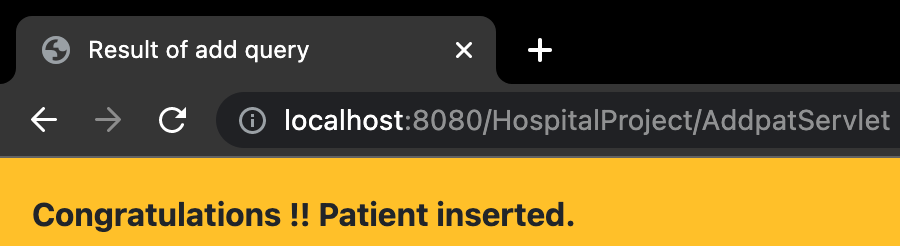
\includegraphics[scale=0.65]{screenshots/2j.png}
    \label{fig:my_label1}
    \caption{Successful insertion of patient}
\end{figure}

\begin{figure}[!hbt]
    \centering
    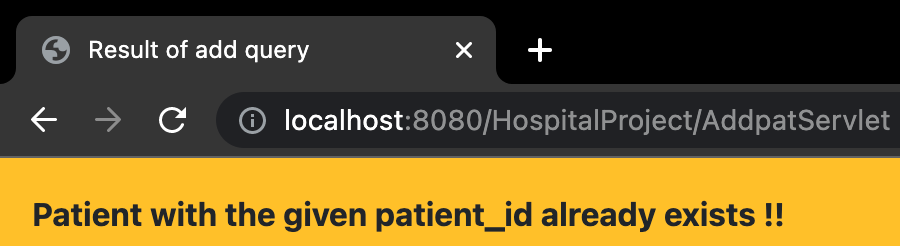
\includegraphics[scale=0.65]{screenshots/2k.png}
    \label{fig:data}
    \caption{Error message if we try to violate the PK constraint}
\end{figure}

\newpage

\begin{figure}[!hbt]
    \centering
    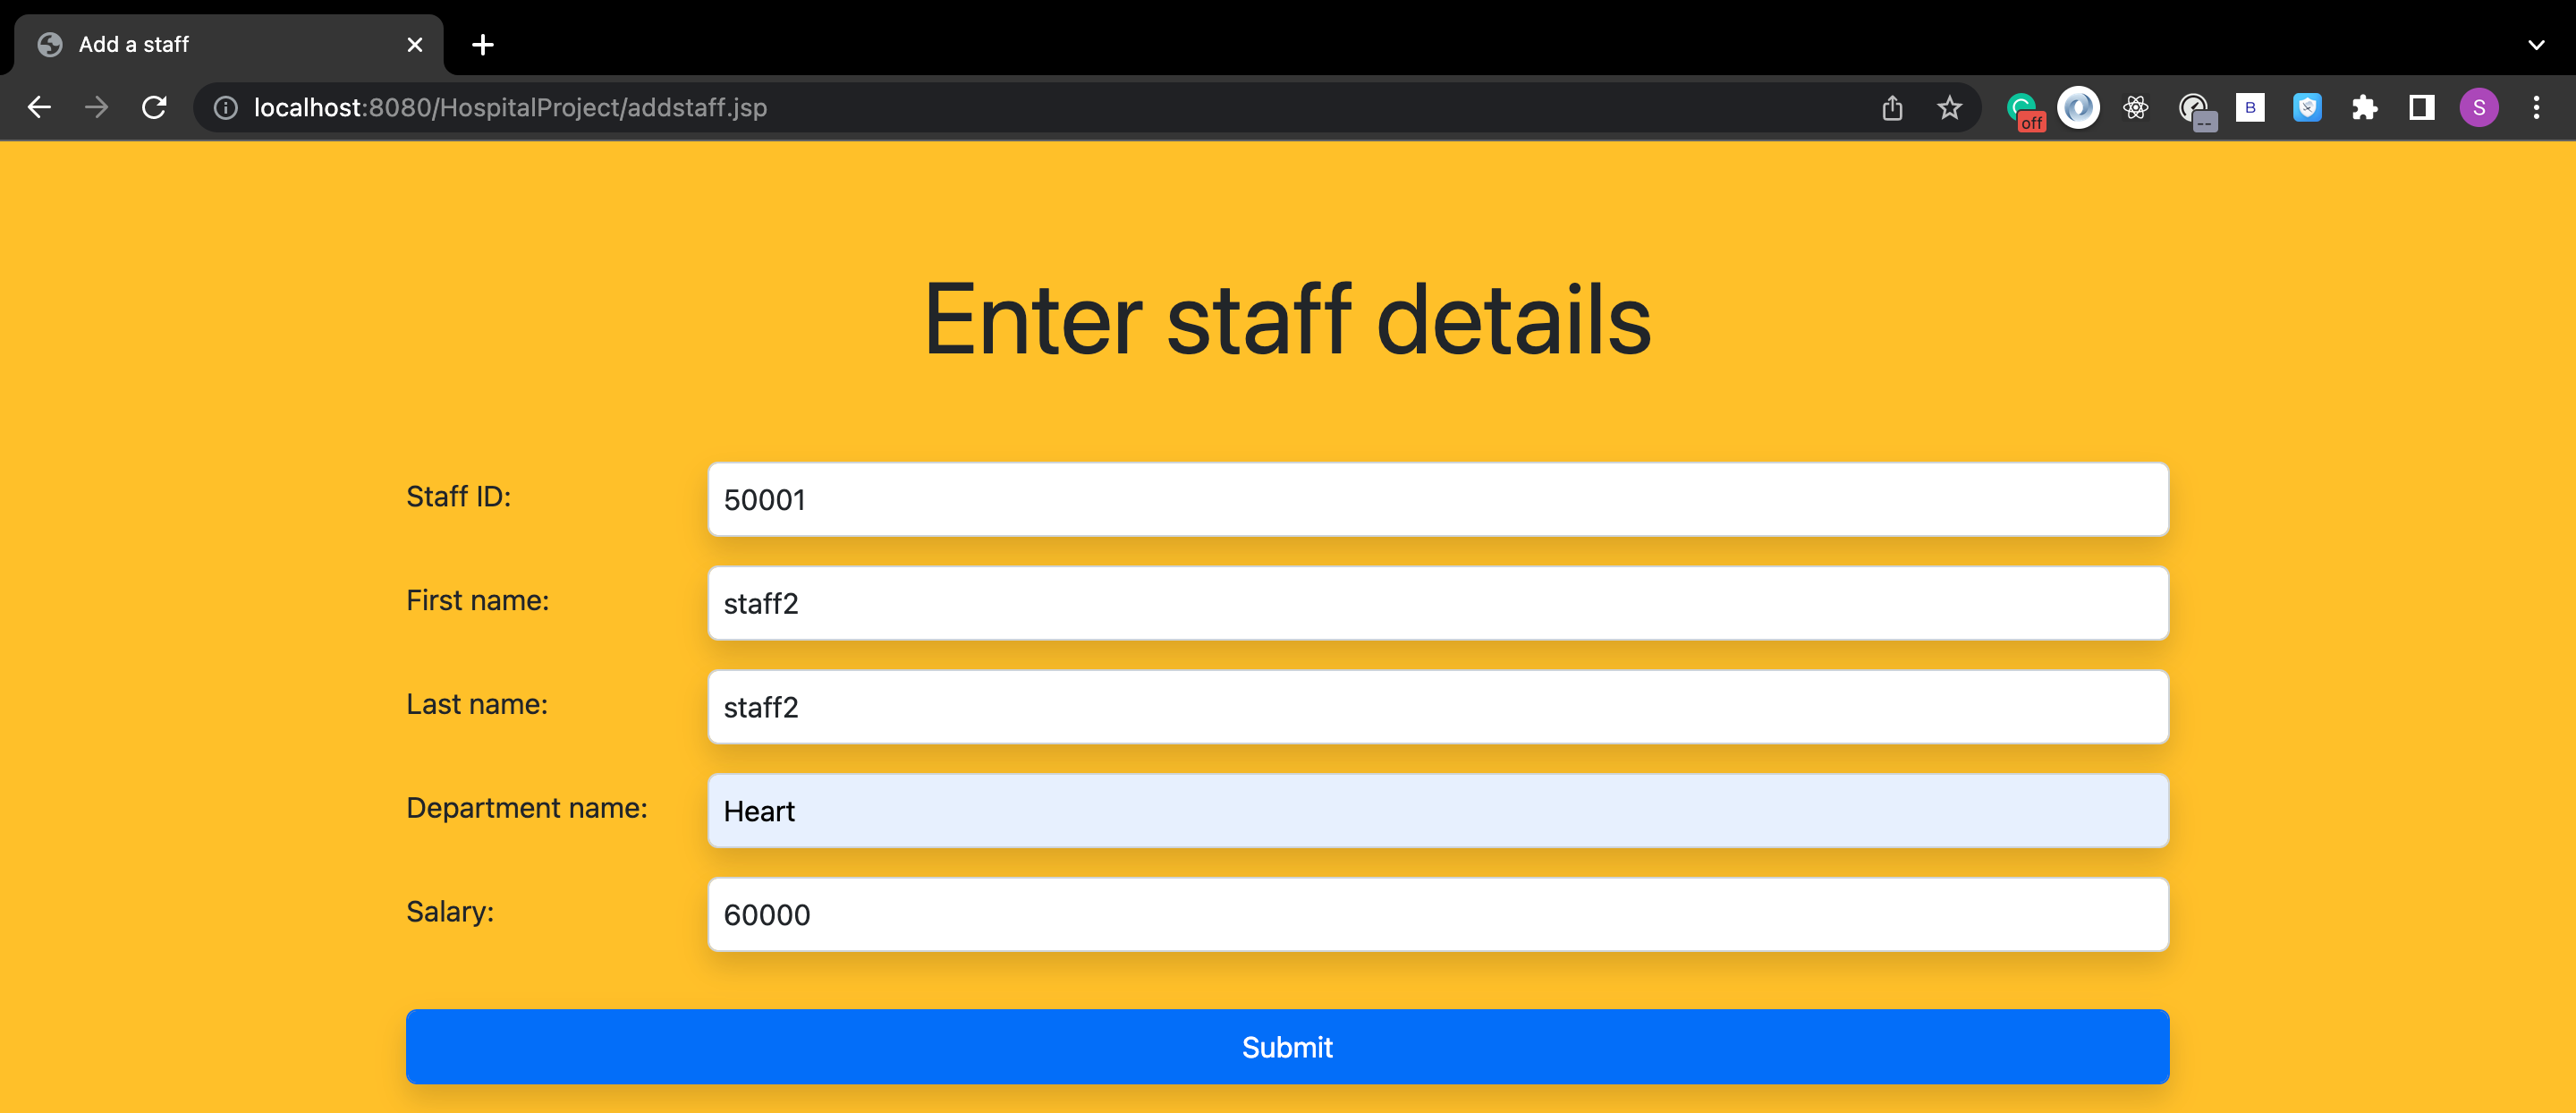
\includegraphics[scale=0.35]{screenshots/2l.png}
    \label{fig:my_label1}
    \caption{Adding a staff}
\end{figure}

\begin{figure}[!hbt]
    \centering
    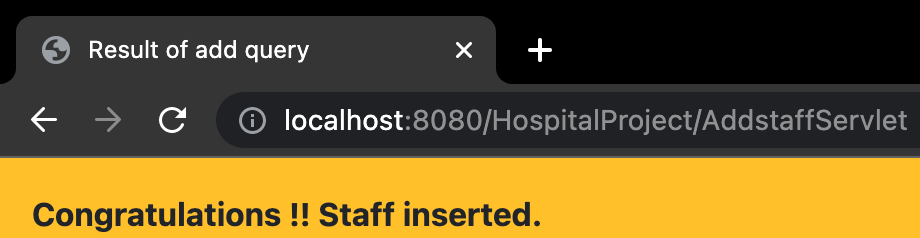
\includegraphics[scale=0.85]{screenshots/2m.png}
    \label{fig:data}
    \caption{Successful insertion of staff}
\end{figure}

\begin{figure}[!hbt]
    \centering
    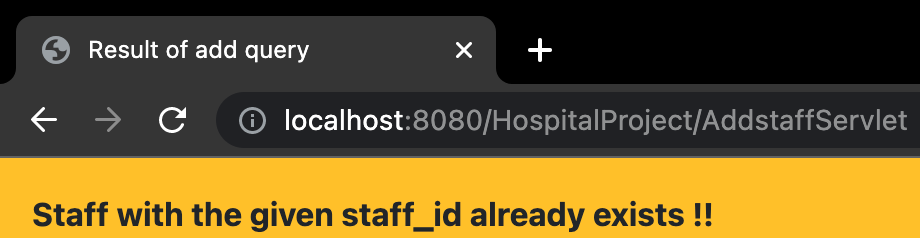
\includegraphics[scale=0.85]{screenshots/2n.png}
    \label{fig:my_label1}
    \caption{Error message if we try to violate the PK constraint}
\end{figure}

\newpage

\begin{figure}[!hbt]
    \centering
    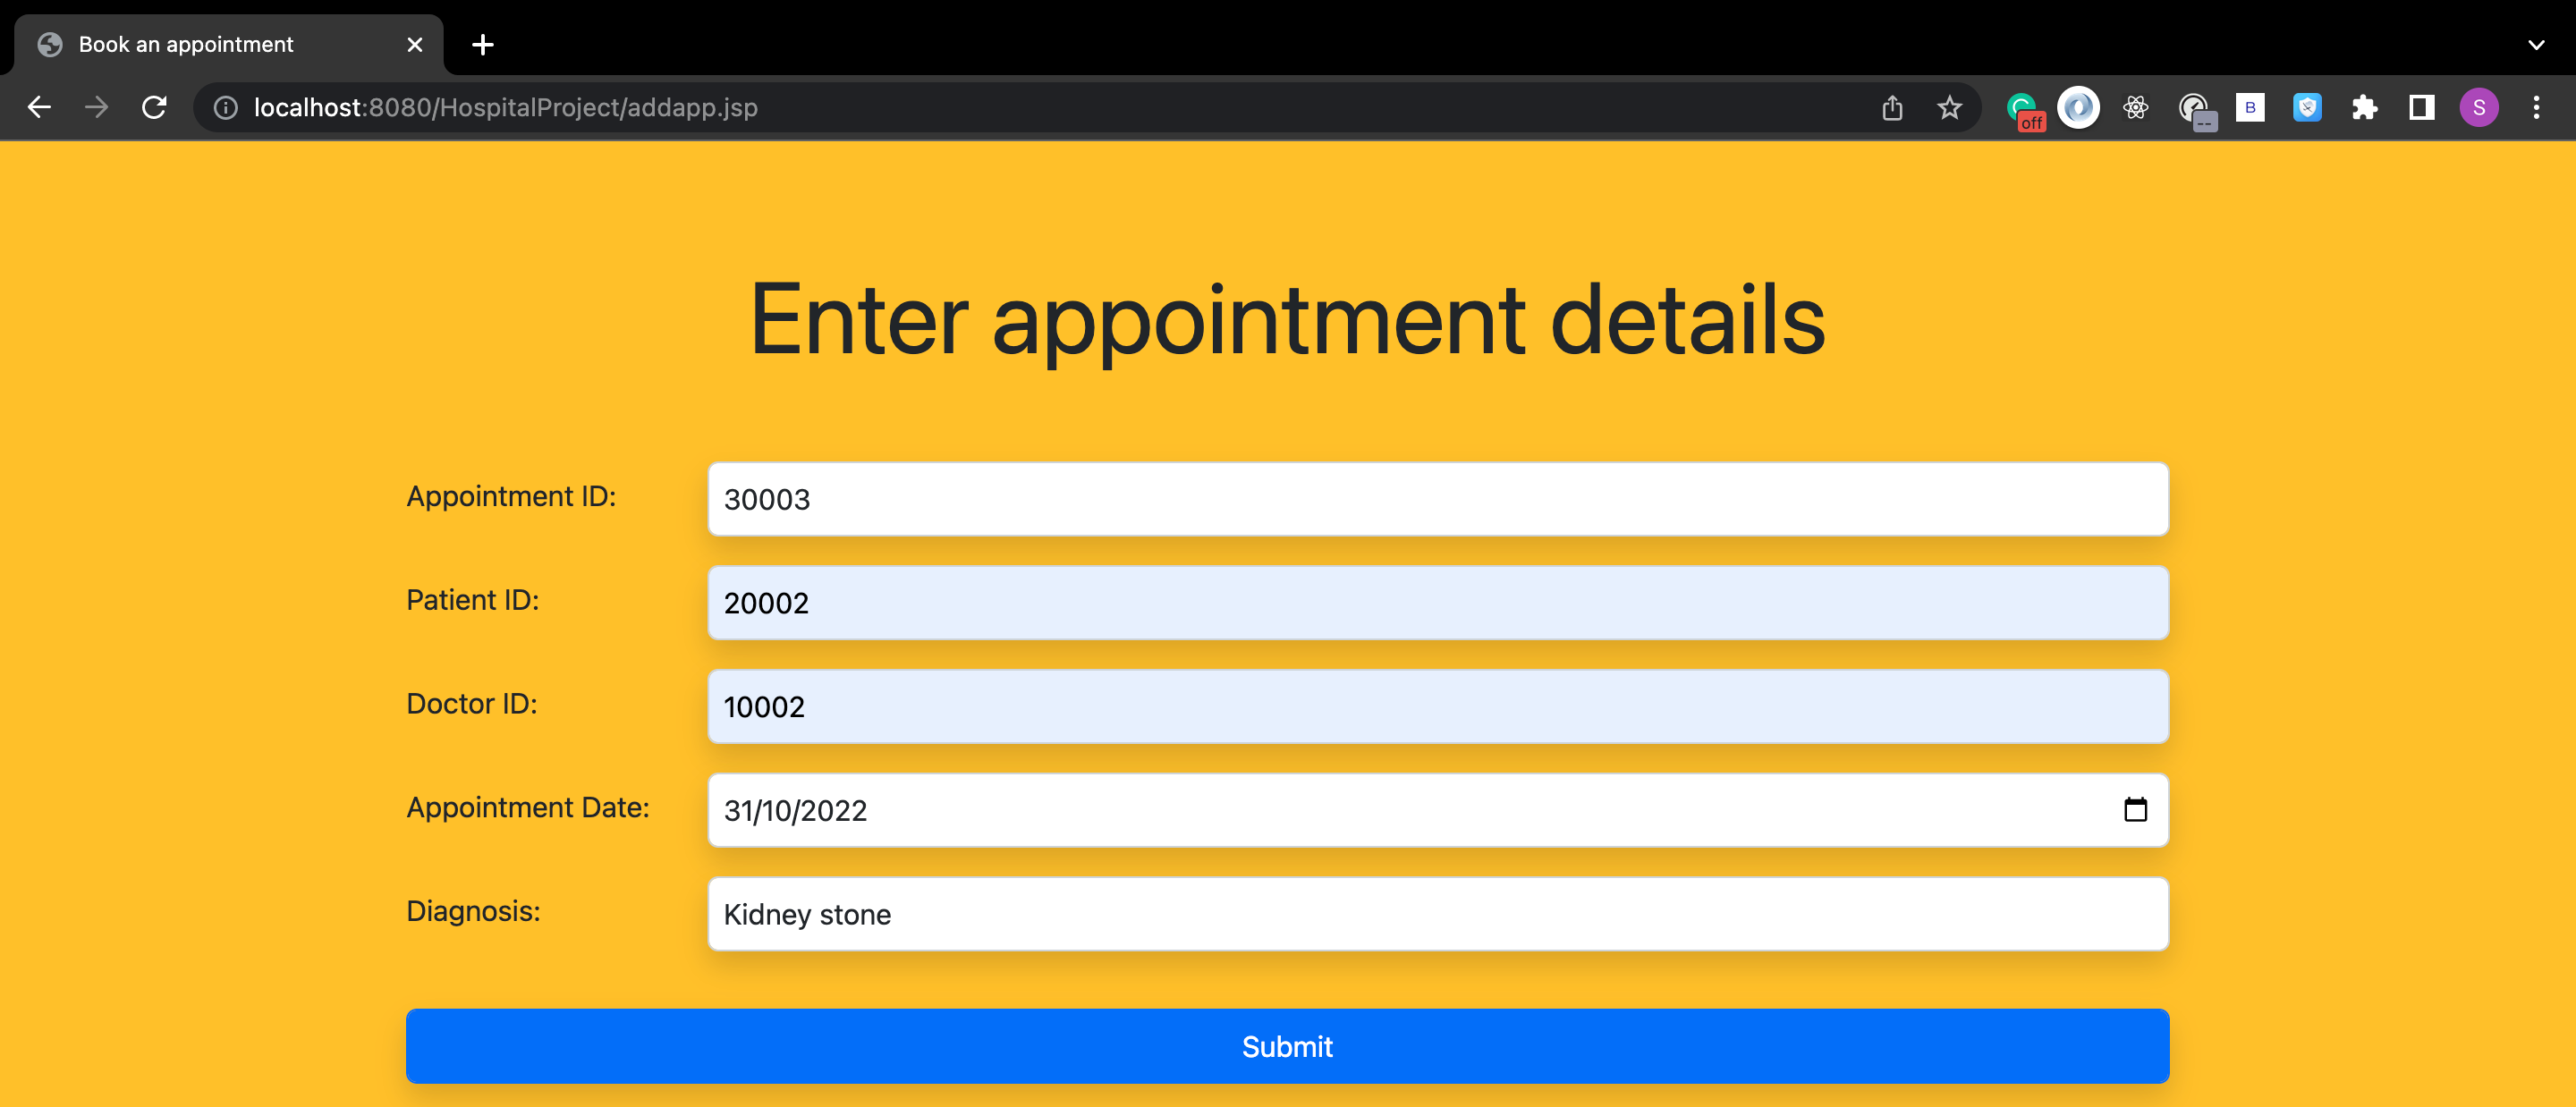
\includegraphics[scale=0.35]{screenshots/2o.png}
    \label{fig:data}
    \caption{Booking an appointment (by admin)}
\end{figure}

\begin{figure}[!hbt]
    \centering
    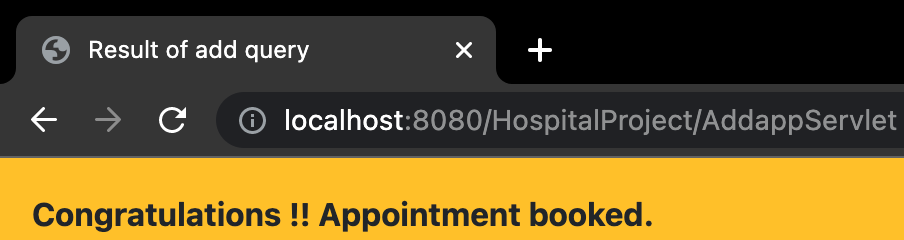
\includegraphics[scale=0.9]{screenshots/2p.png}
    \label{fig:my_label1}
    \caption{Successful booking}
\end{figure}

\begin{figure}[!hbt]
    \centering
    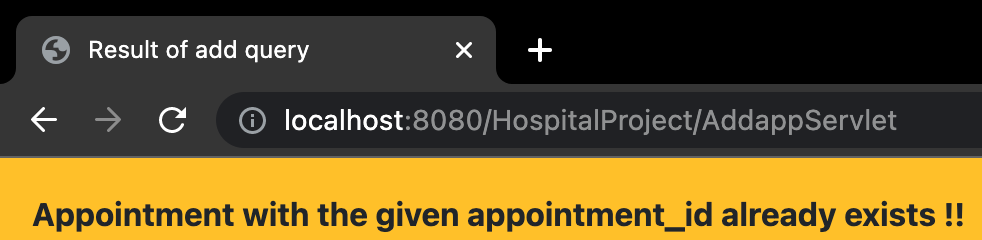
\includegraphics[scale=0.9]{screenshots/2q.png}
    \label{fig:data}
    \caption{Error message if we try to violate the PK constraint}
\end{figure}

\newpage

\begin{figure}[!hbt]
    \centering
    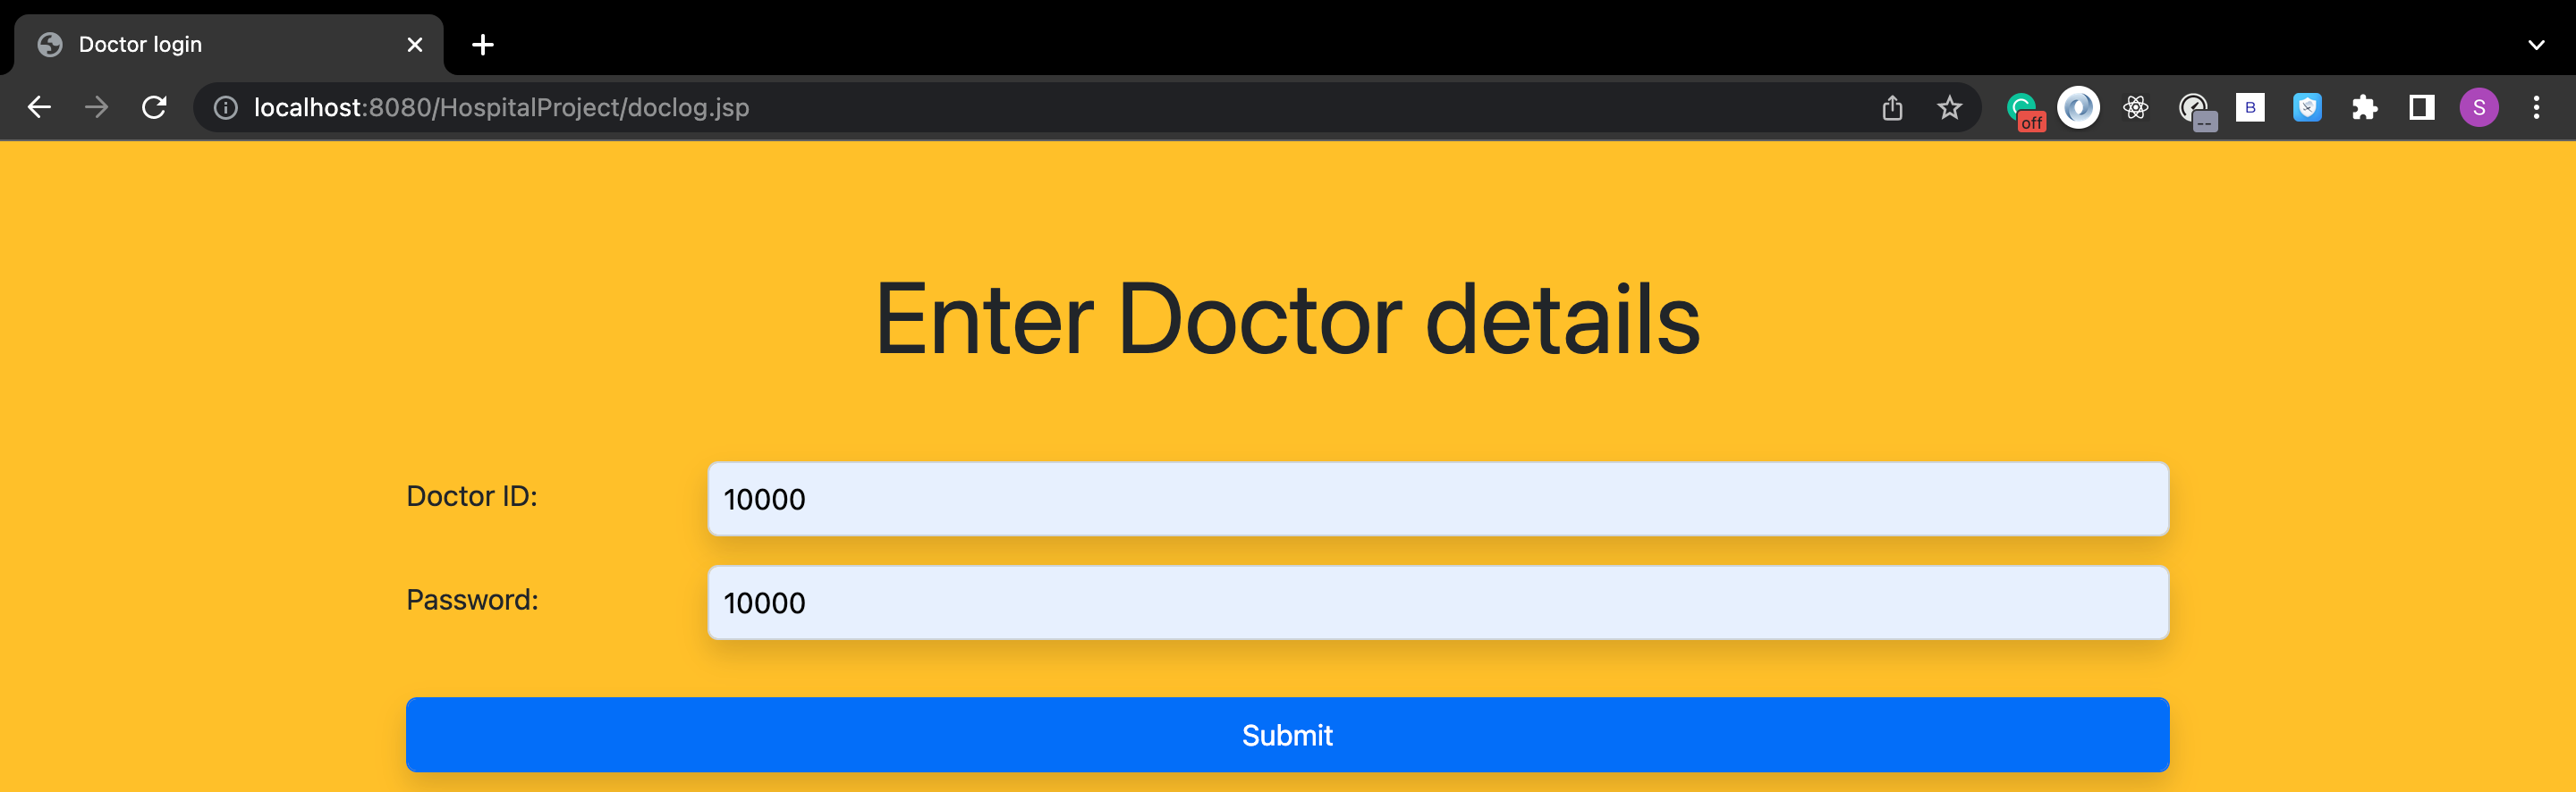
\includegraphics[scale=0.35]{screenshots/3a.png}
    \label{fig:my_label1}
    \caption{Doctor login page(using correct credentials)}
\end{figure}

\vspace{15mm}

\begin{figure}[!hbt]
    \centering
    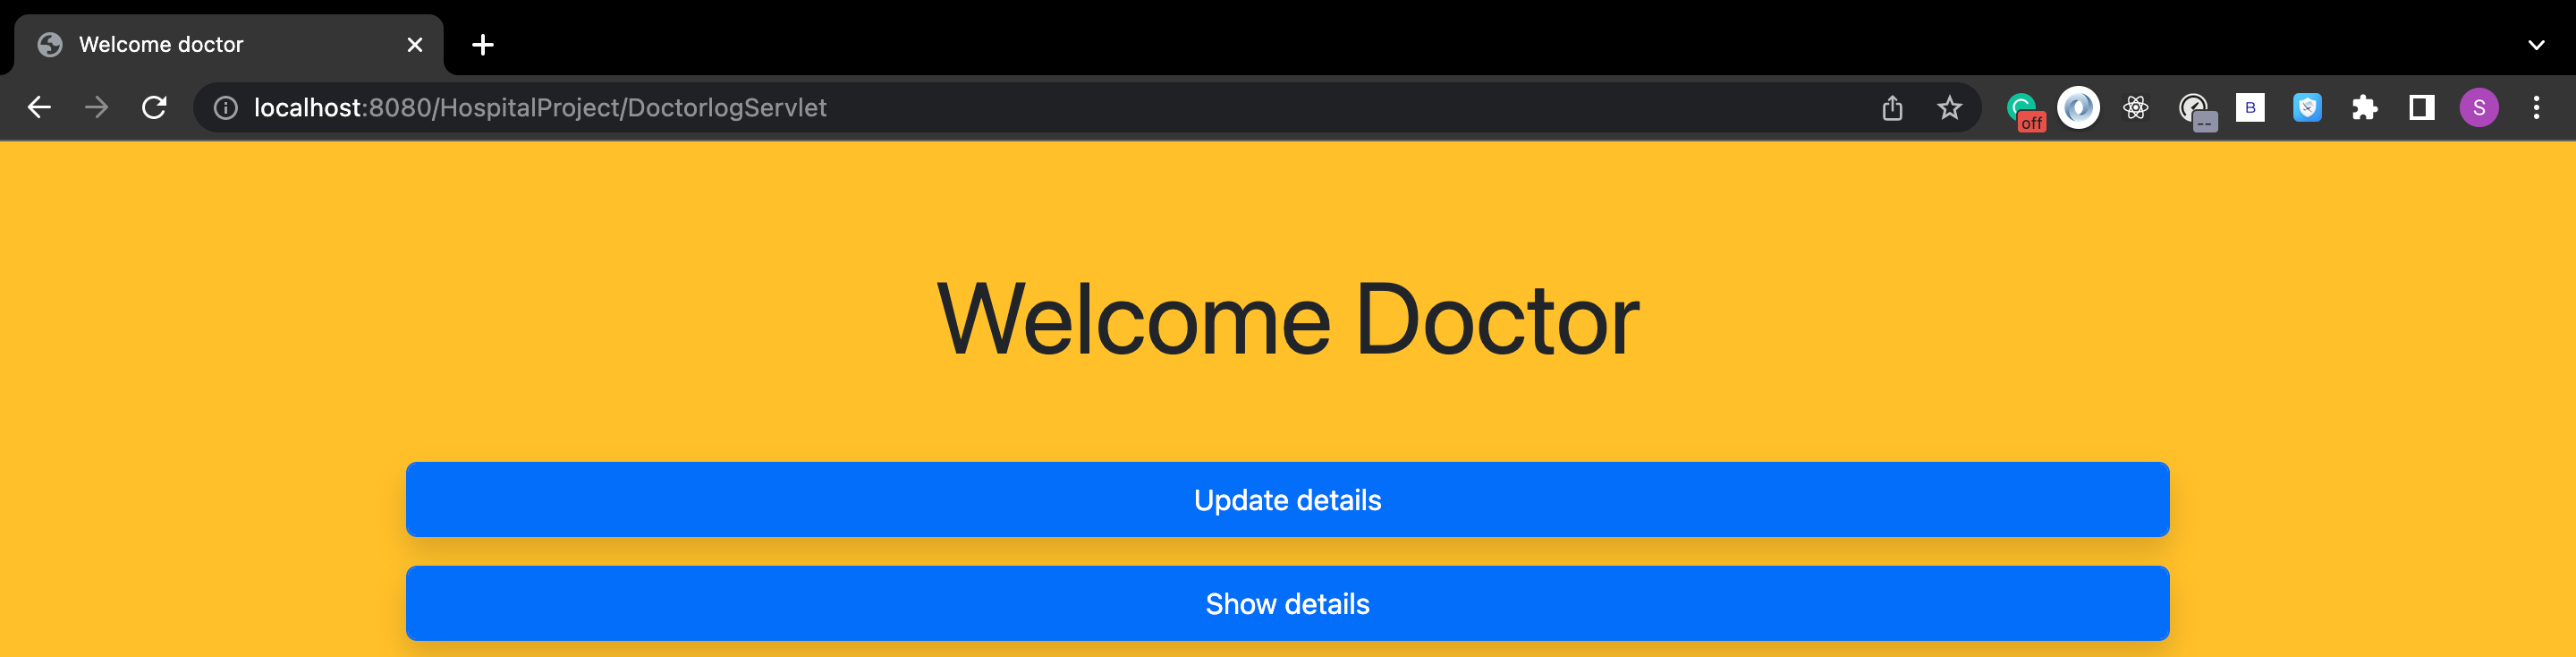
\includegraphics[scale=0.35]{screenshots/3b.png}
    \label{fig:data}
    \caption{Page after successful doctor login}
\end{figure}

\newpage

\begin{figure}[!hbt]
    \centering
    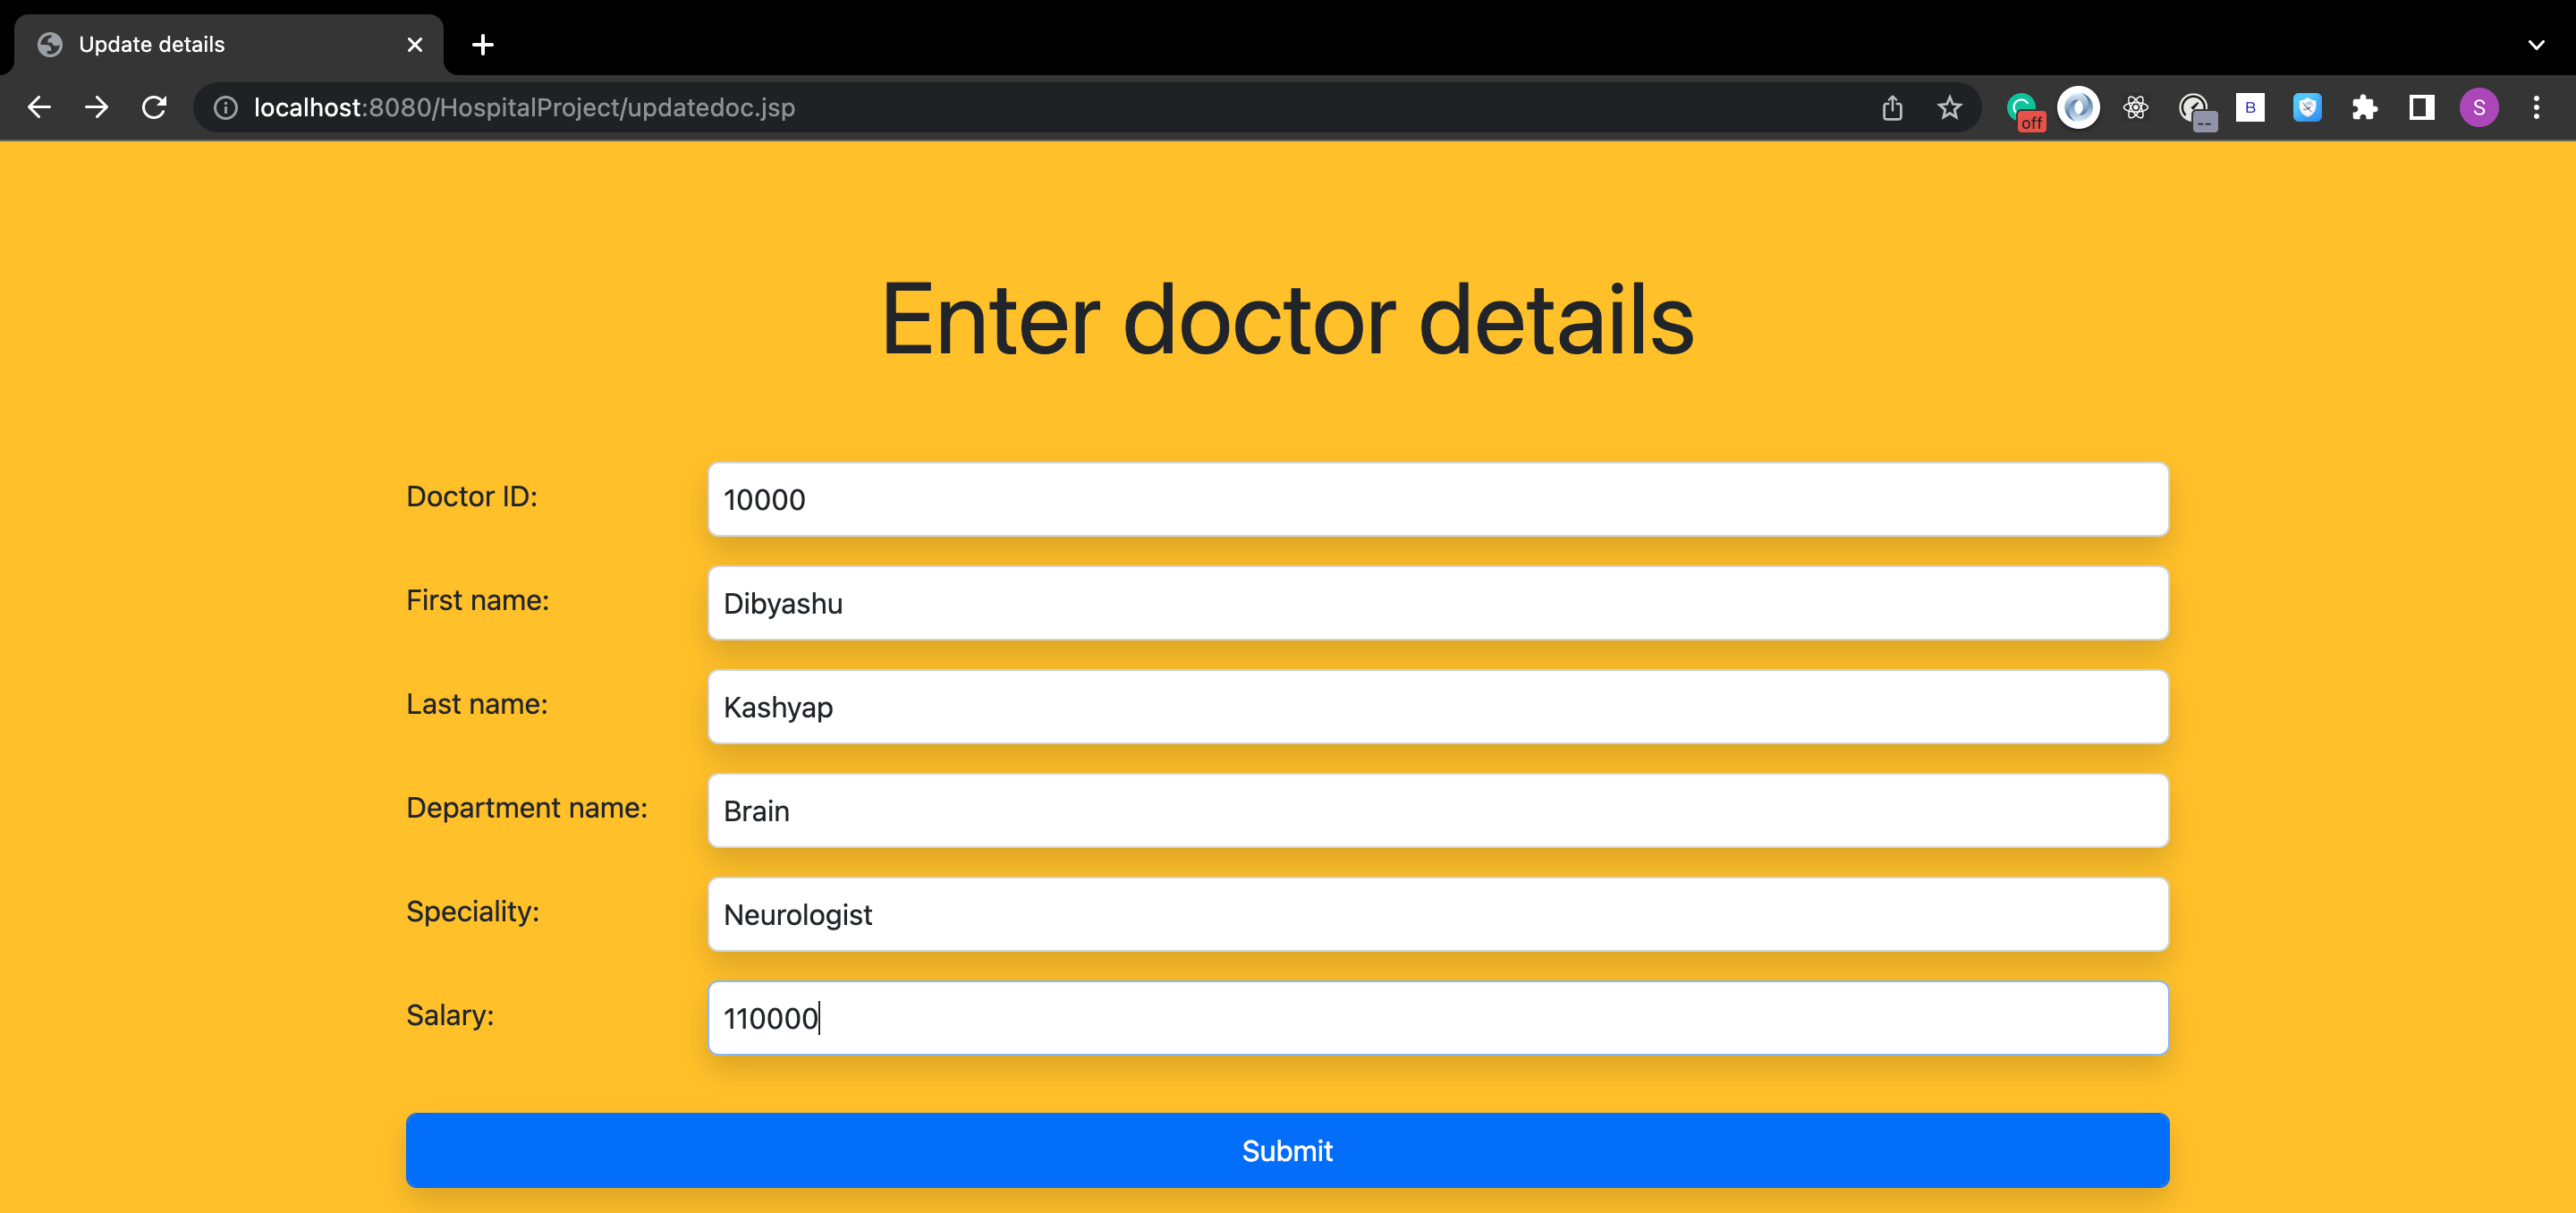
\includegraphics[scale=0.35]{screenshots/3c.png}
    \label{fig:my_label1}
    \caption{Updating doctor details}
\end{figure}

\vspace{15mm}

\begin{figure}[!hbt]
    \centering
    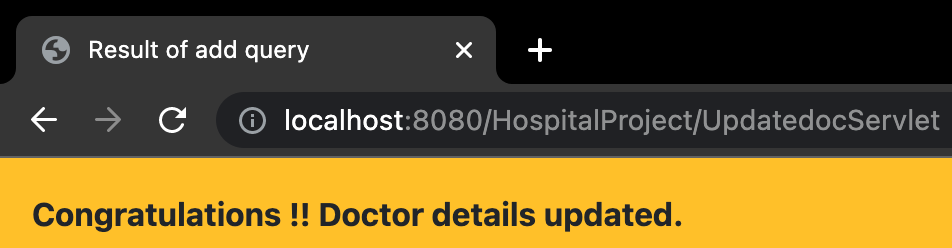
\includegraphics[scale=0.9]{screenshots/3d.png}
    \label{fig:data}
    \caption{Result of update query}
\end{figure}

\newpage

\begin{figure}[!hbt]
    \centering
    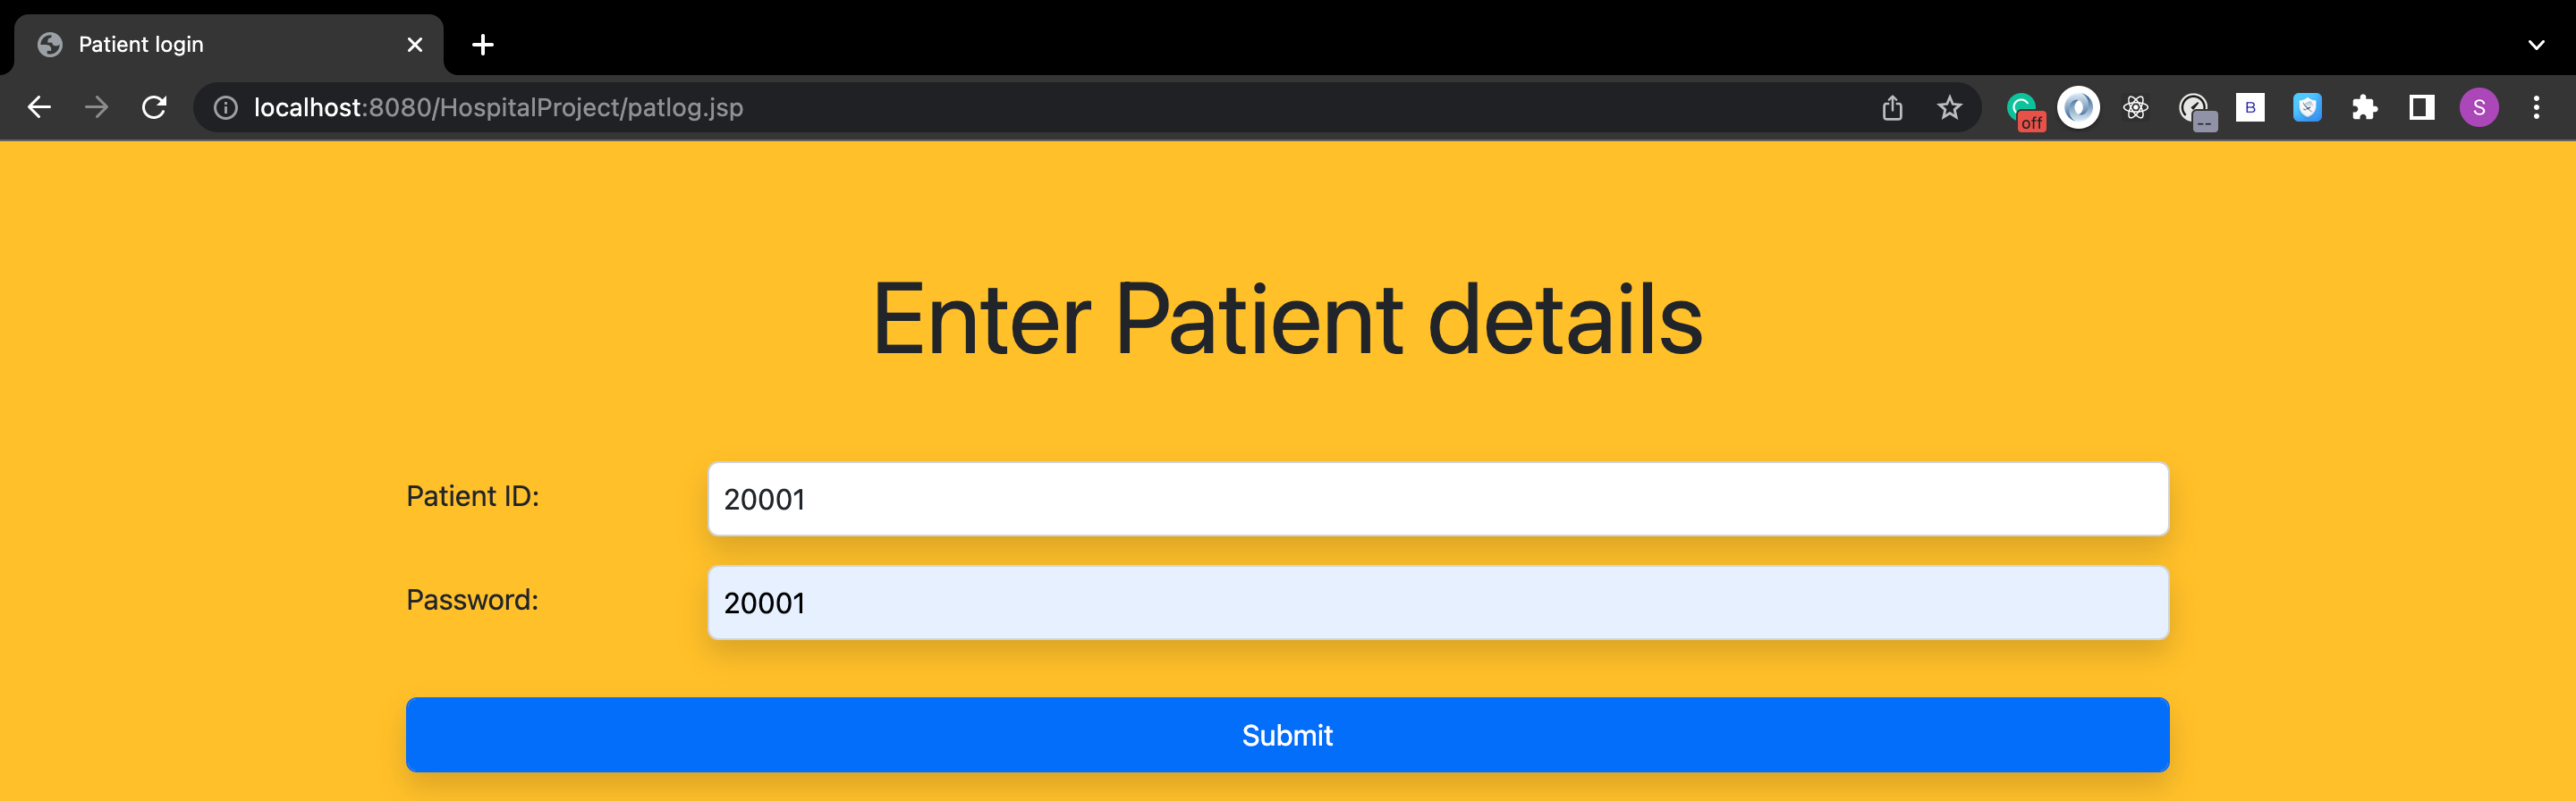
\includegraphics[scale=0.35]{screenshots/4a.png}
    \label{fig:my_label1}
    \caption{Patient login page(using correct credentials)}
\end{figure}

\vspace{15mm}

\begin{figure}[!hbt]
    \centering
    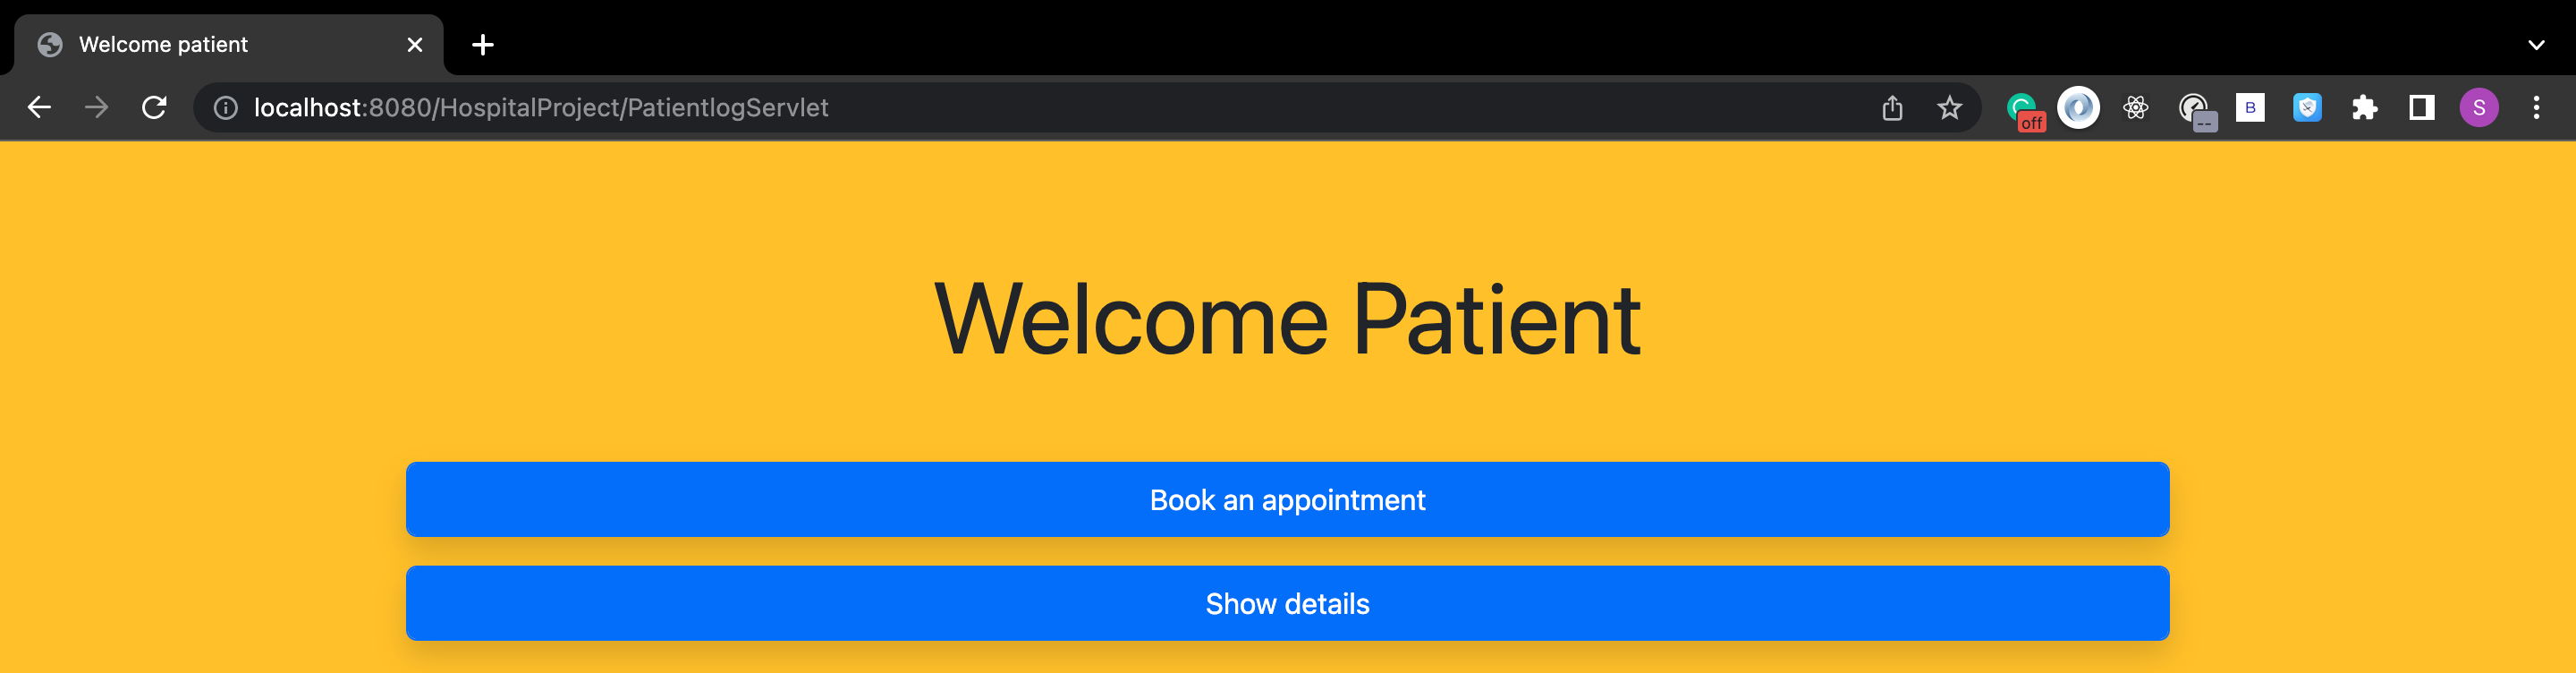
\includegraphics[scale=0.35]{screenshots/4b.png}
    \label{fig:data}
    \caption{Page after successful patient login}
\end{figure}

\newpage

\begin{figure}[!hbt]
    \centering
    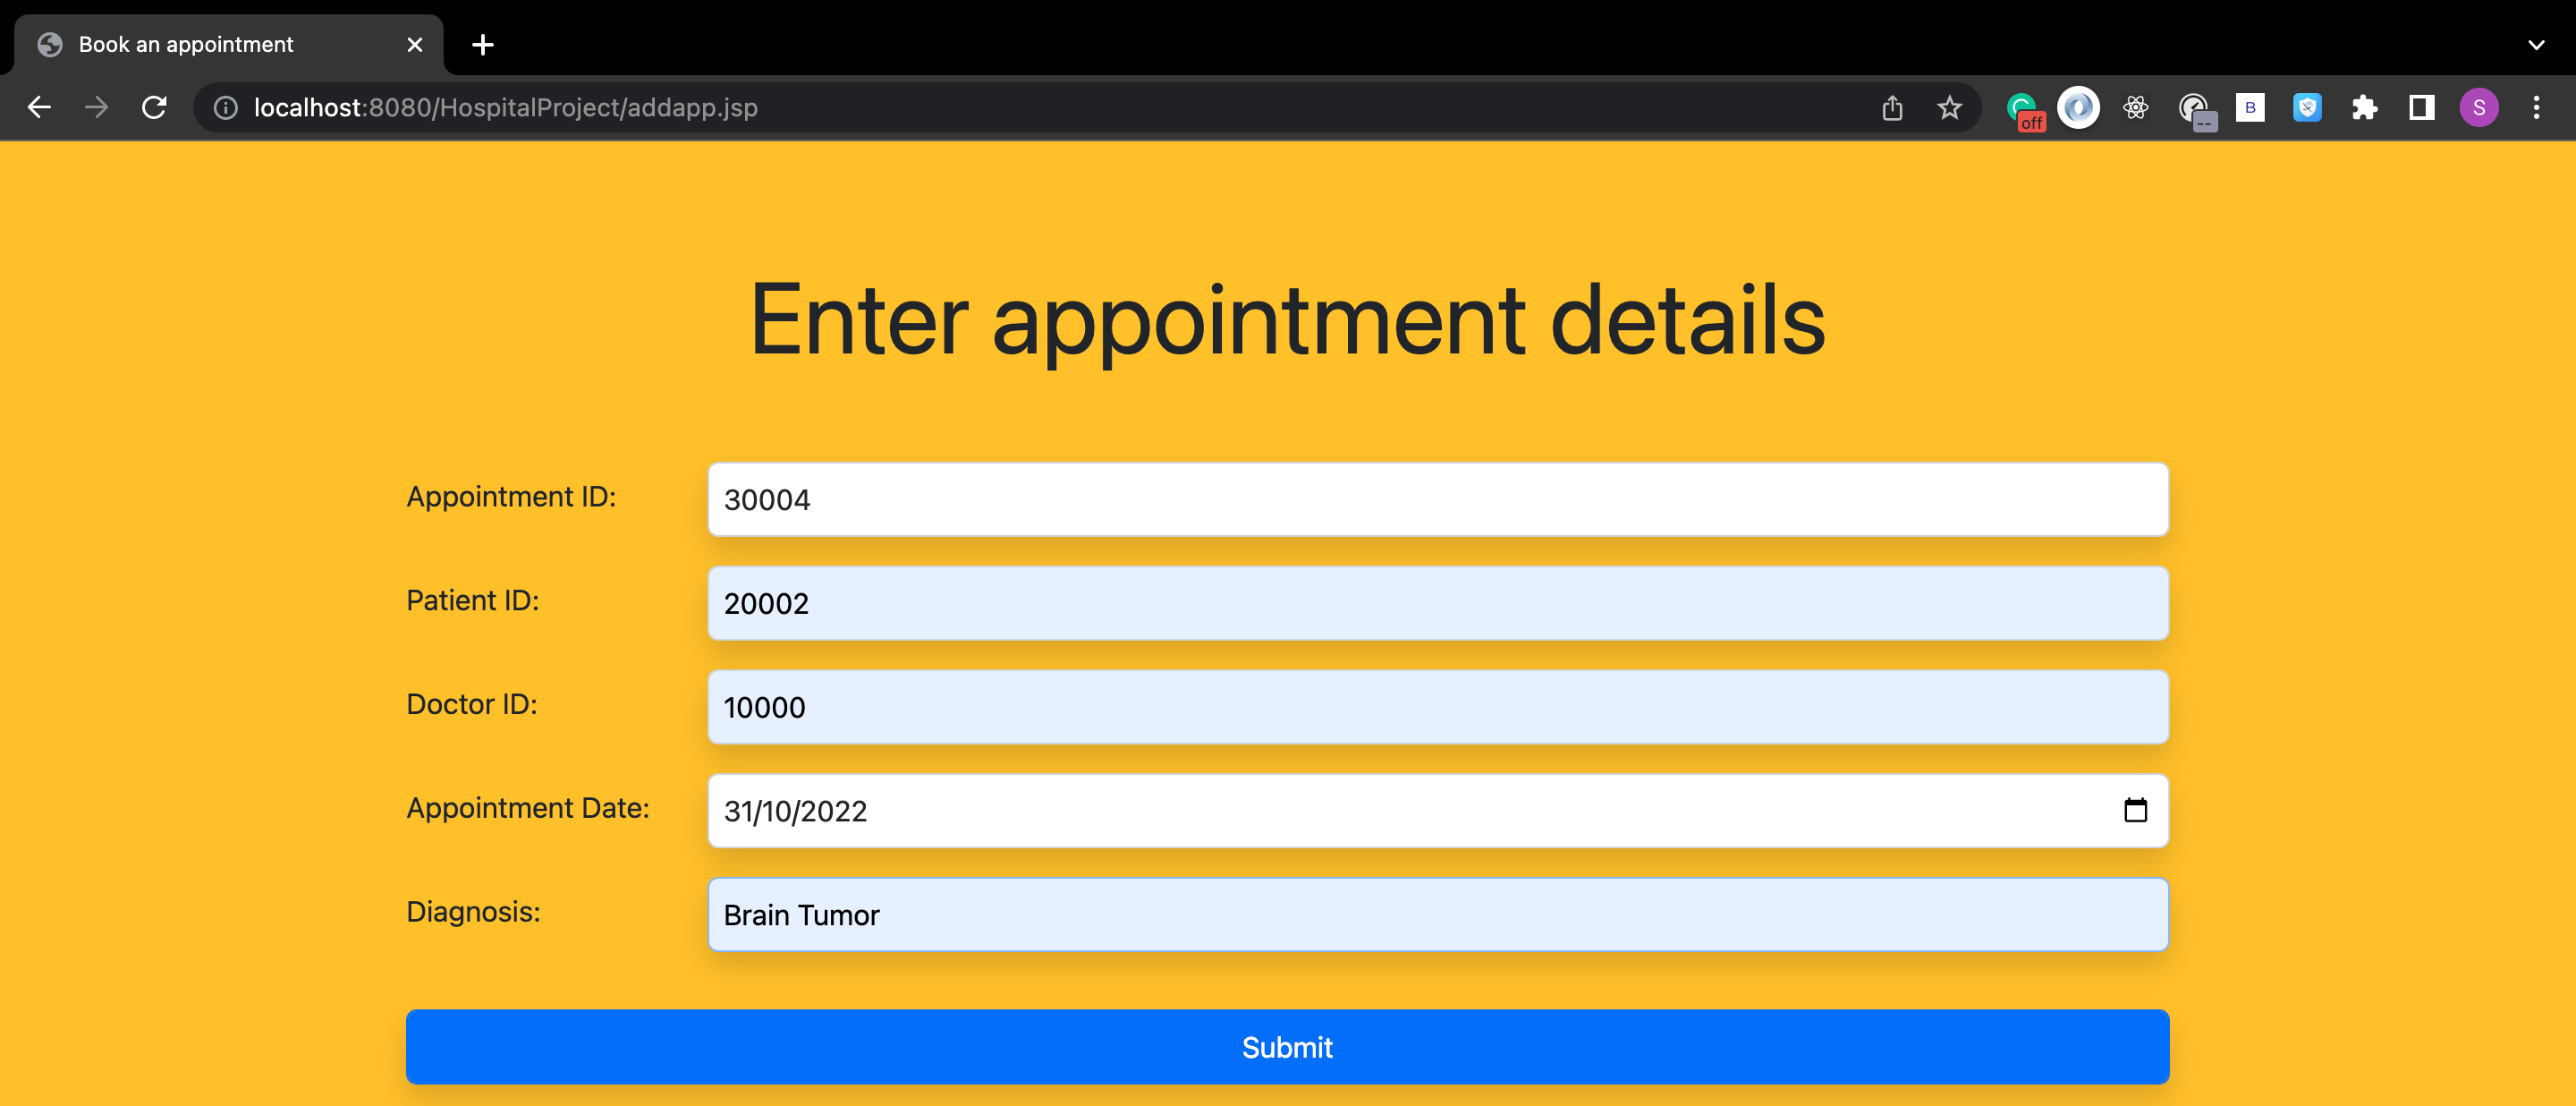
\includegraphics[scale=0.35]{screenshots/4c.png}
    \label{fig:my_label1}
    \caption{Booking an appointment (by patient) }
\end{figure}

\begin{figure}[!hbt]
    \centering
    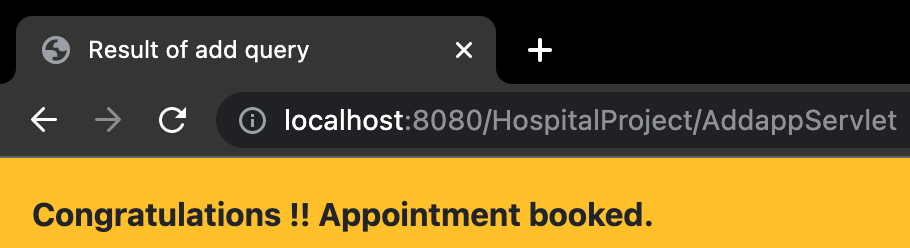
\includegraphics[scale=0.9]{screenshots/4d.png}
    \label{fig:data}
    \caption{Successful booking}
\end{figure}

\begin{figure}[!hbt]
    \centering
    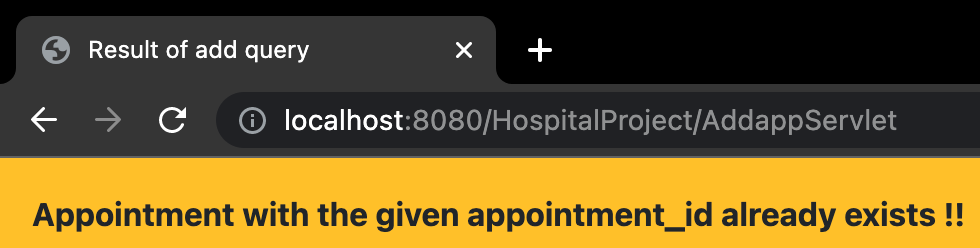
\includegraphics[scale=0.9]{screenshots/4e.png}
    \label{fig:my_label1}
    \caption{Error message if we try to violate the PK constraint}
\end{figure}

\newpage

\begin{figure}[!hbt]
    \centering
    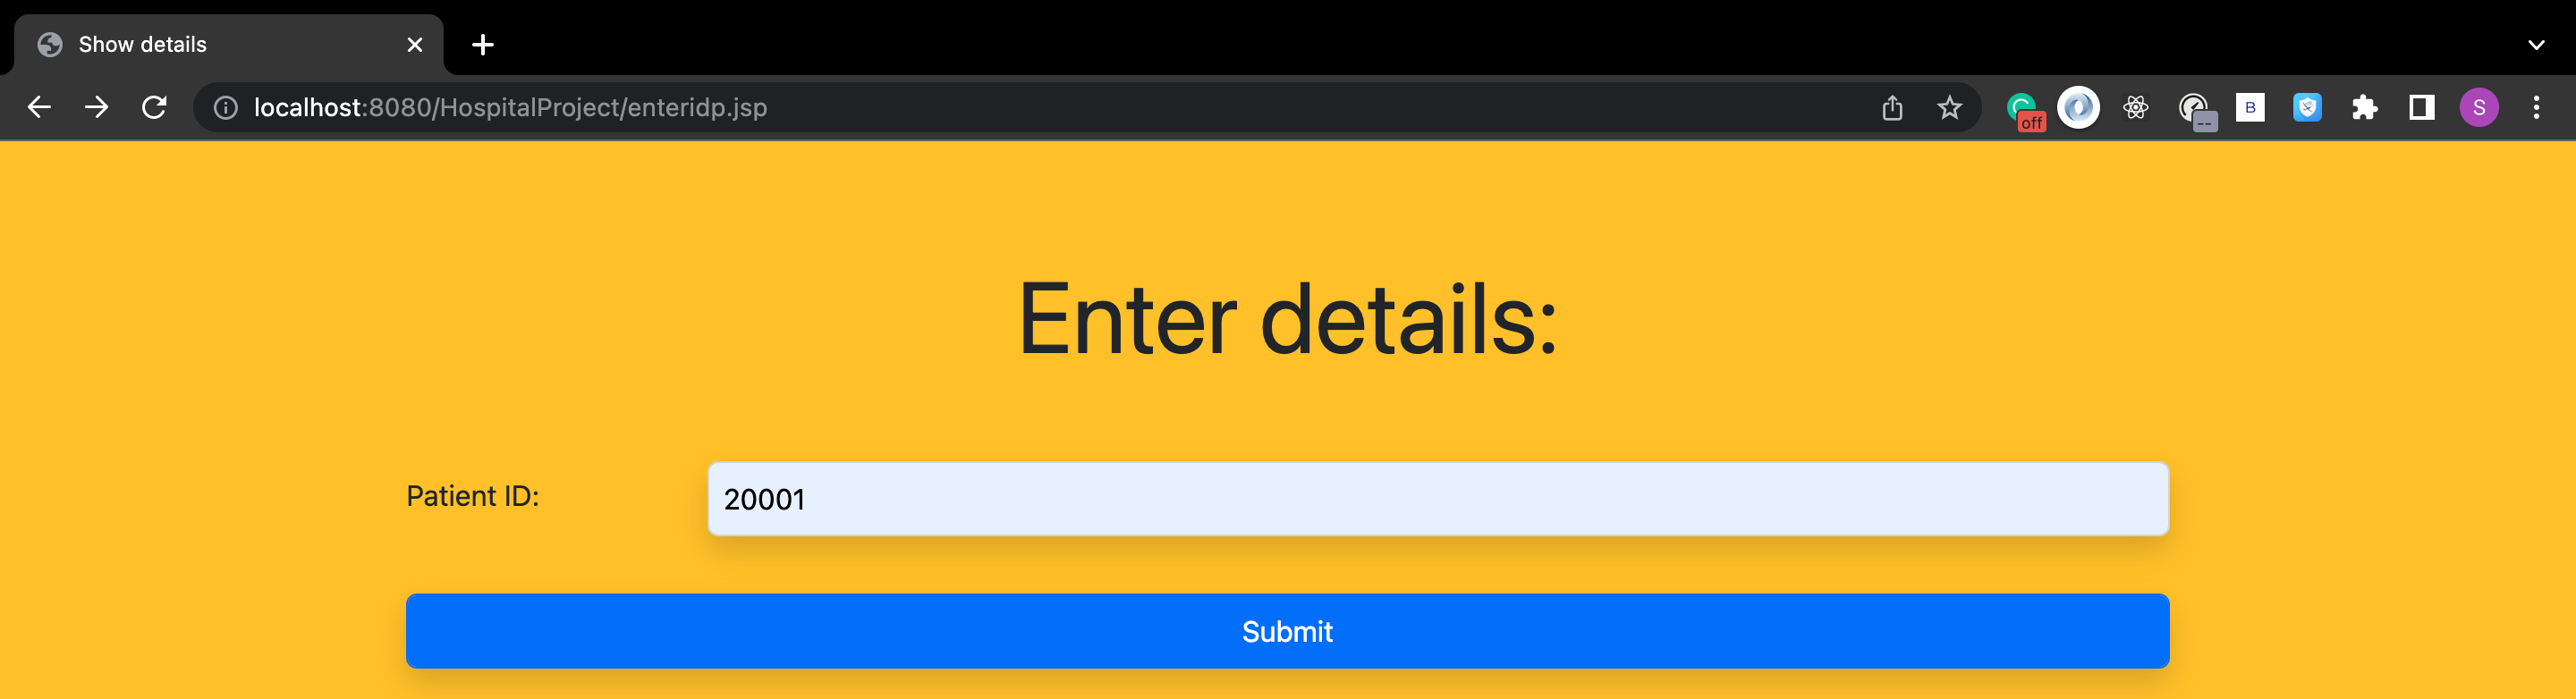
\includegraphics[scale=0.35]{screenshots/6a.png}
    \label{fig:data}
    \caption{Page for entering id for showing details}
\end{figure}

\vspace{15mm}

\begin{figure}[!hbt]
    \centering
    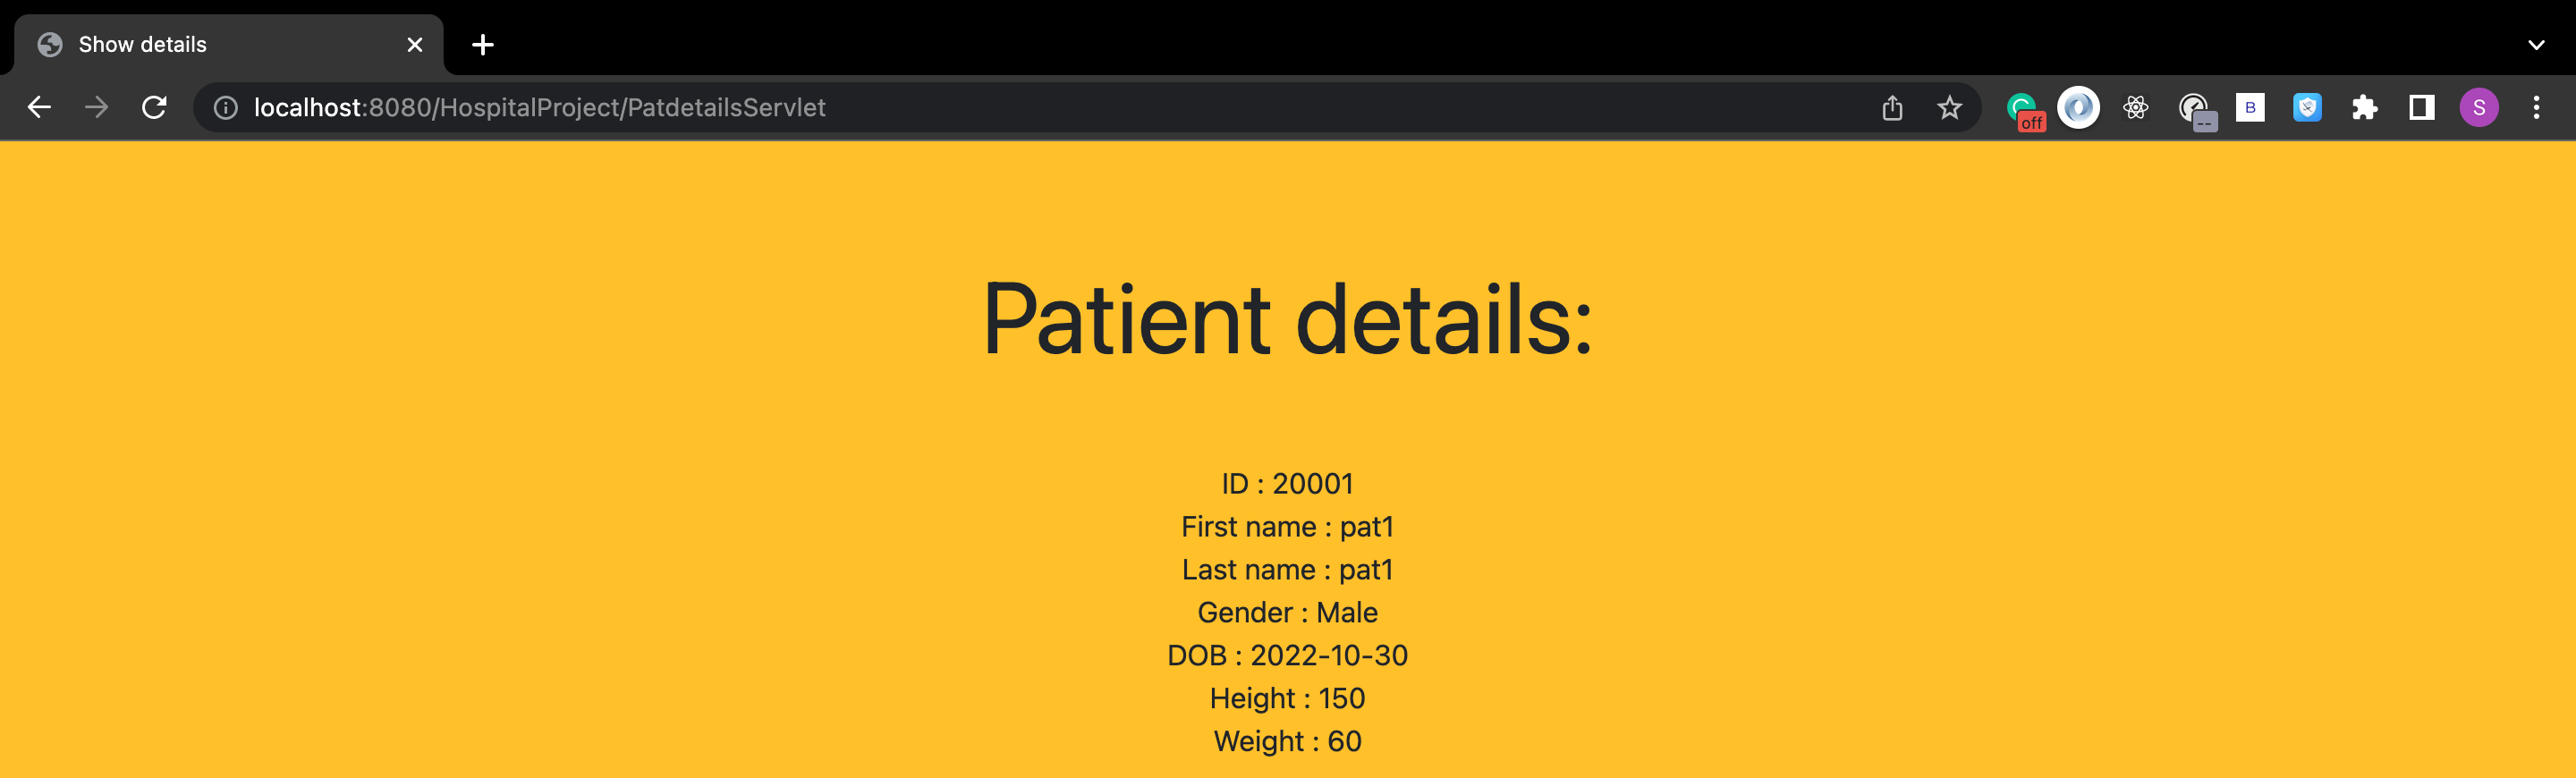
\includegraphics[scale=0.35]{screenshots/6b.png}
    \label{fig:my_label1}
    \caption{Viewing patient details}
\end{figure}

\newpage

\begin{figure}[!hbt]
    \centering
    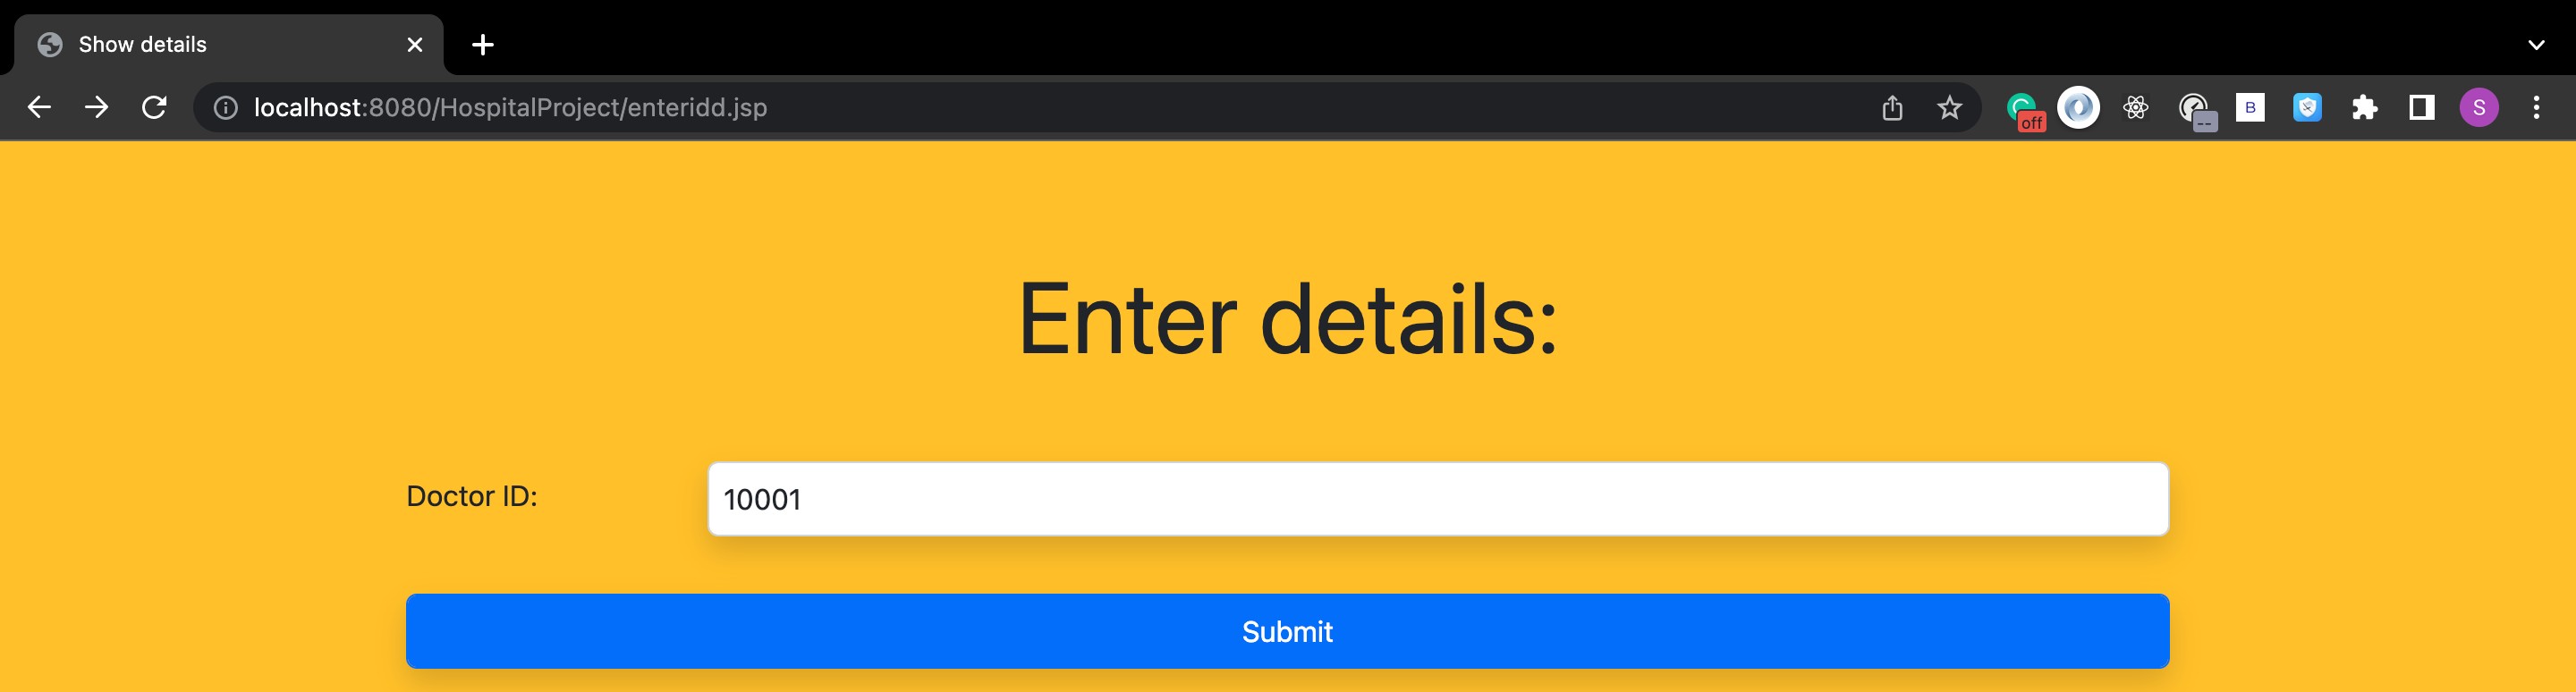
\includegraphics[scale=0.35]{screenshots/6c.png}
    \label{fig:data}
    \caption{Page for entering id for showing details}
\end{figure}

\vspace{15mm}

\begin{figure}[!hbt]
    \centering
    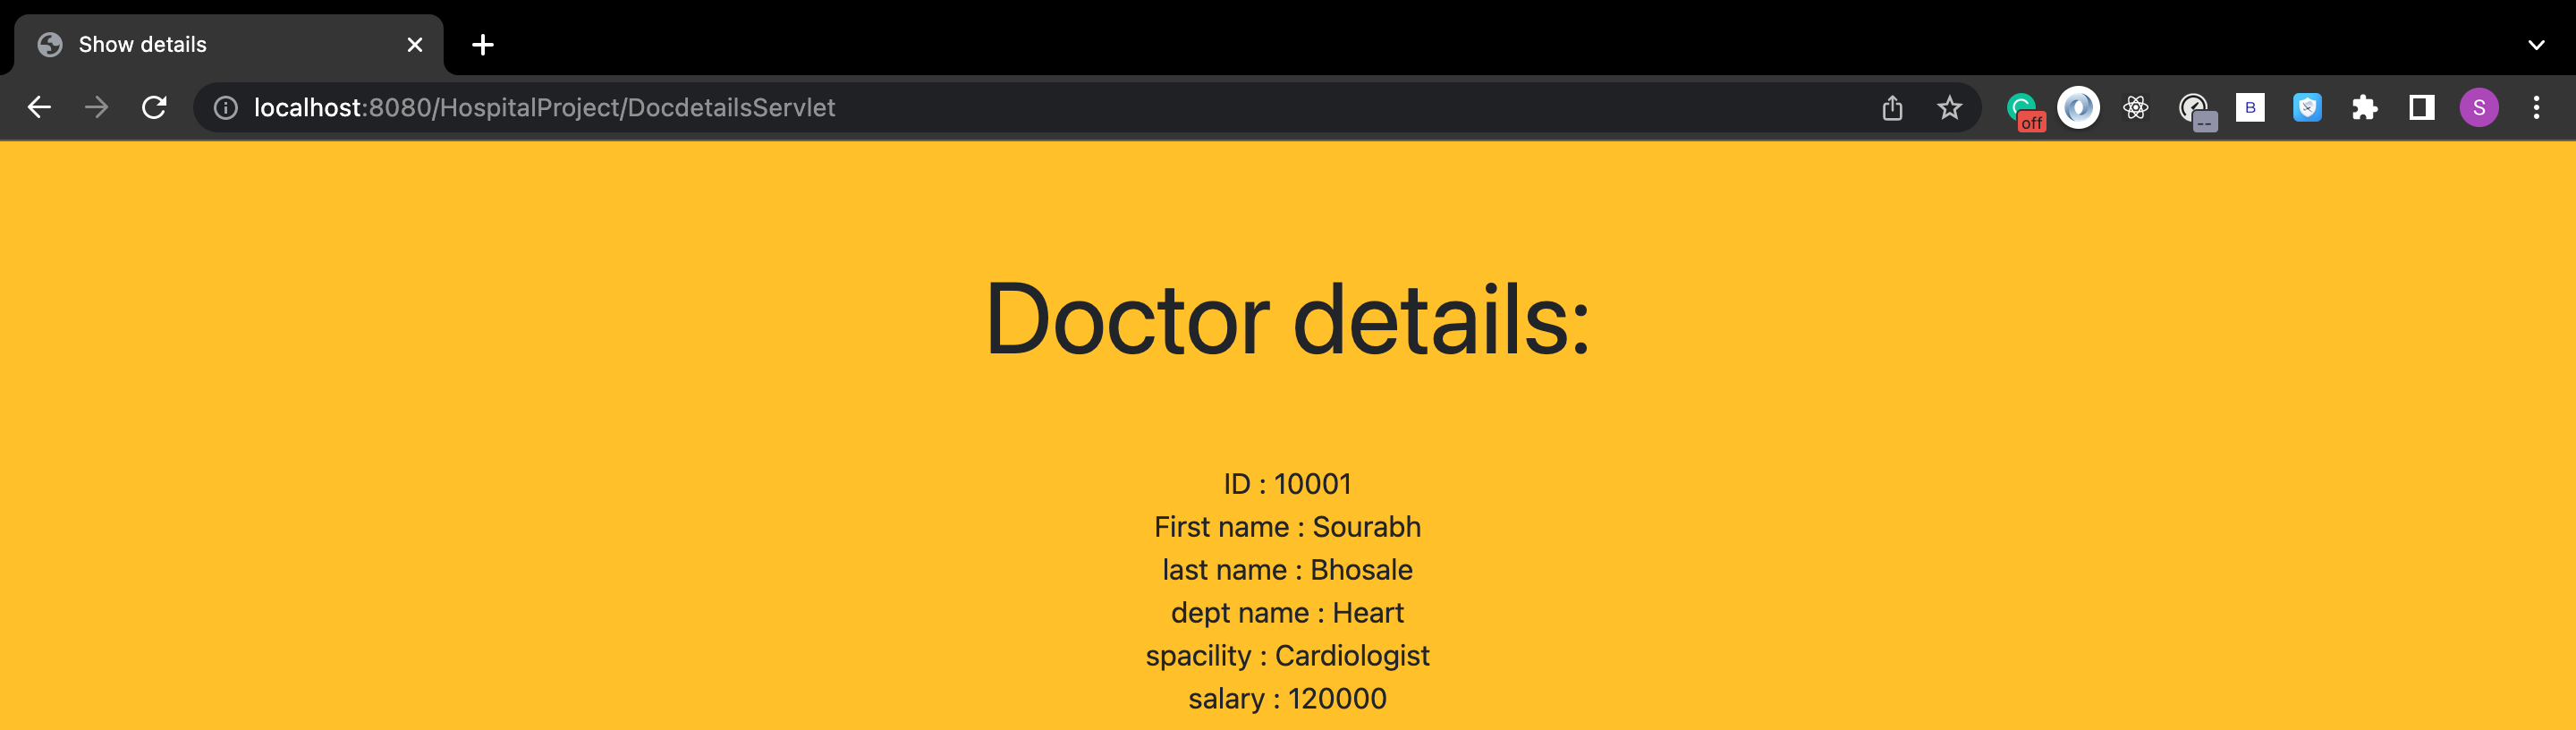
\includegraphics[scale=0.35]{screenshots/6d.png}
    \label{fig:my_label1}
    \caption{Viewing doctor details}
\end{figure}

% \newpage
%---------------------------------------------------------------------
\section{Conclusion}

\setstretch{1.5}
We created an hospital management system that stores hospital data about patients, doctors, staff, appointments , departments and the credentials of involved parties in MySQL database and used JDBC to communicate with MySQL database from Servlets to make our website interactive. This can be used to manage a hospital or a clinic kind of setup that will provide patient with the flexibility to book appointment both with admin (the receptionist at the hospital can act as admin) and at the ease of their home. 

\singlespacing
\newpage


\end{document}